\documentclass{beamer}
\usepackage{ctex}
\usepackage{indentfirst}
\usepackage{hyperref}
\usepackage{graphicx}
\usepackage{caption}
\usepackage{subfigure}
\usetheme{CambridgeUS}
\author{HJQwQ}
\title{题目讲评}
\date{2020年8月16日}
\setlength{\parindent}{2em}
\begin{document}
	\frame{\titlepage}
	\begin{frame}\frametitle{目录}
		\tableofcontents
	\end{frame}
	\section{多米诺骨牌}
		\subsection{各种部分分}
			\begin{frame}\frametitle{测试点1}
				$n=1,m\le10$\\
				显然n=1的时候用$1\times2$的骨牌尽可能靠左填就行
			\end{frame}
			\begin{frame}\frametitle{测试点2,3}
				$n\le2,m\le10^5$\\
				显然n=2的时候用$2\times1$的骨牌尽可能靠左填就行
			\end{frame}
			\begin{frame}\frametitle{测试点4,5}
				$n\le5,m\le10^5$\\
				说实话我也没想过这部分该怎么做..可能有乱搞能拿50分\\
				但其实我小小地卡了一下我能想到的几种贪心乱搞..乱搞能过的话算你狠
			\end{frame}
			\begin{frame}\frametitle{测试点6,7}
				$n\le10,m\le1000$\\
				这部分或许可以用插头DP来做..但写起来肯定会很恶心所以我也没细想..
			\end{frame}
		\subsection{正解}
			\begin{frame}\frametitle{一个结论}
				答案就是$\lfloor\frac{(n+1)(m+1)}6\rfloor$\\
				惊不惊喜?刺不刺激?(仿佛梦回NOIP2017D1T1)
			\end{frame}
		\subsection{证明}
			\begin{frame}\frametitle{问题转化}
				原问题是在$n\times m$的棋盘中,放入若干\textbf{不相邻}的$1\times2$或$2\times1$的骨牌\\
				这个问题等价于在$(n+1)\times(m+1)$的棋盘中,放入若干\textbf{不重叠}的$2\times3$或$3\times2$的骨牌\\
				我们不难证明这两个问题中的方案是一一对应的:在第二个问题的任一个方案中,所有的骨牌删去最上方一行和最左侧一列,再删去棋盘的最上方一行和最左侧一列,就能得到第一个问题的一种方案\\
				类似地,在第一个问题的任一个方案中,所有的骨牌在左侧添加一列,在上方添加一行,再在整个棋盘的最左侧添加一列,最上方添加一行,就能得到第二个问题的一种方案\\
				故两个问题中能放置骨牌的最大数目相同,这样我们就完成了对问题的转化
			\end{frame}
			\begin{frame}\frametitle{良心插图}
				\begin{figure}[htbp]
					\centering
					\begin{minipage}[t]{0.49\textwidth}
						\centering
						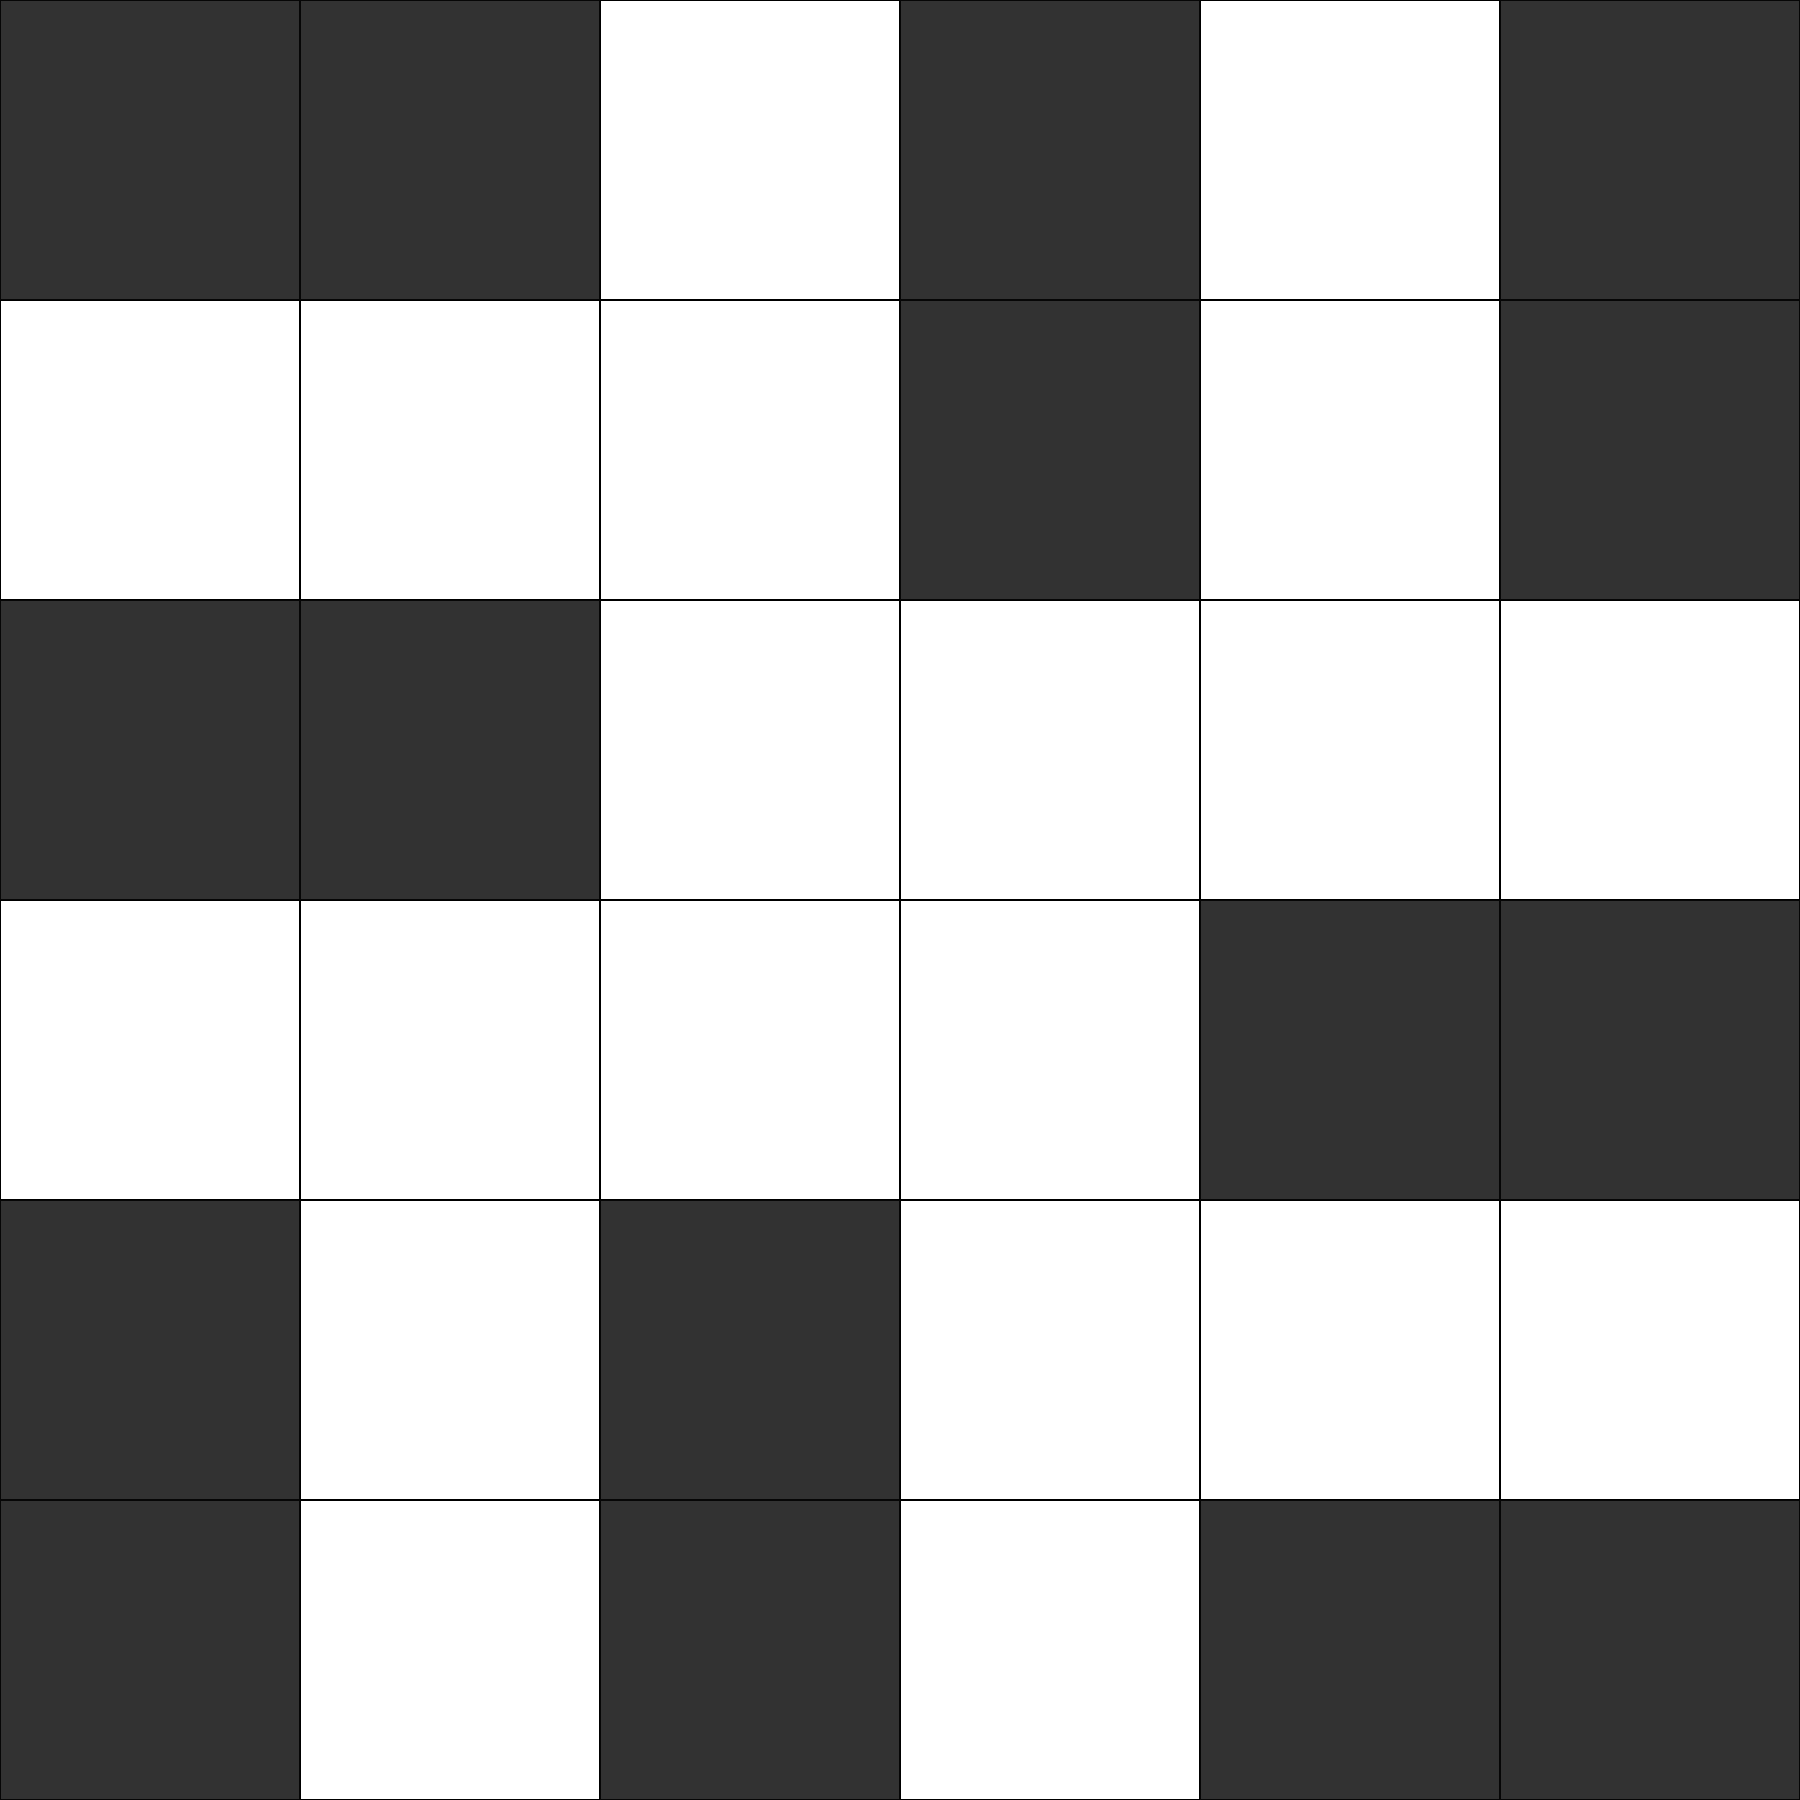
\includegraphics[width=0.6\textwidth]{pictures/1-1.png}
					\end{minipage}
					\begin{minipage}[t]{0.49\textwidth}
						\centering
						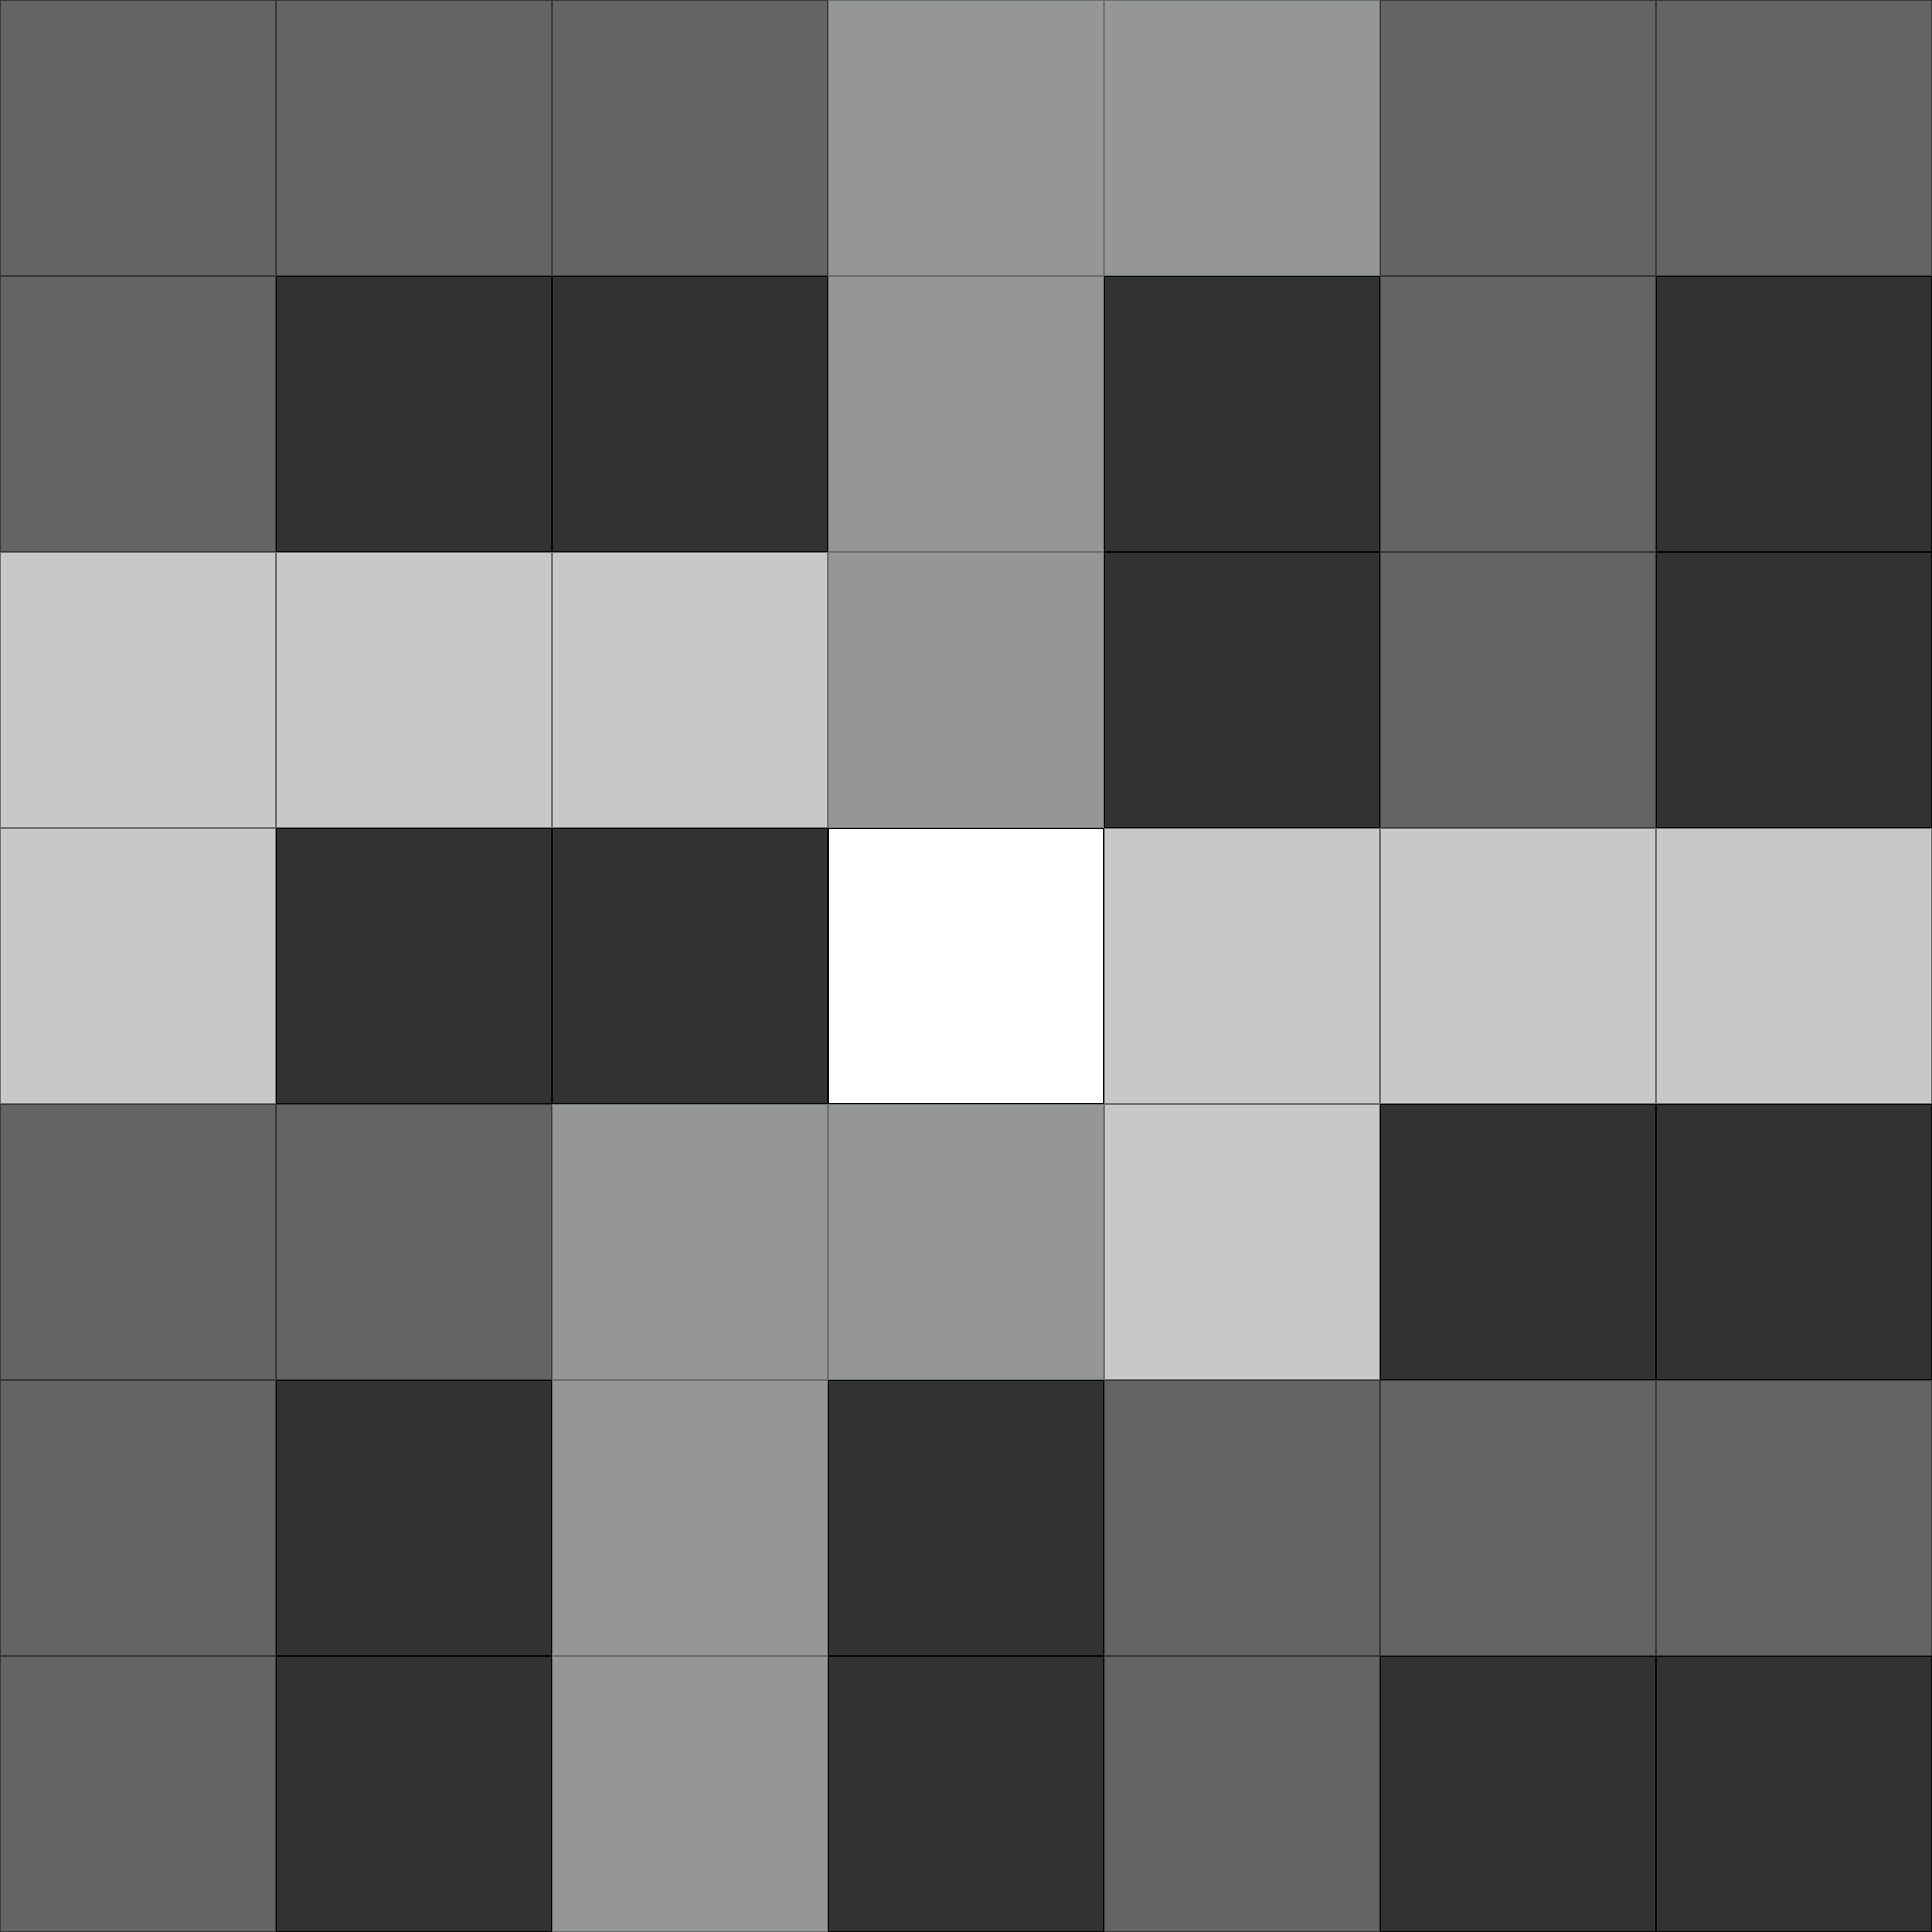
\includegraphics[width=0.7\textwidth]{pictures/1-2.png}
					\end{minipage}
				\end{figure}

				原问题中$n=6,m=6$的最优方案与新问题中的最优方案可相互转化
			\end{frame}
			\begin{frame}\frametitle{$r=2$或$r=3$时..}
				接下来我们讨论的都是转化后的问题\\
				我们将$(n+1)$记作$r$, $(m+1)$记作$c$,故$r,c\ge2$\\
				当$r=2$或$r=3$的时候答案一定是$\lfloor\frac{rc}6\rfloor$,因为我们只要把骨牌挨着放就行了
			\end{frame}
			\begin{frame}\frametitle{$r=6$时}
				结论:当$r=6$时,一定可以放满\\
				首先不难发现当$r=c=6$时,一定是可以放满的,所以只需要按$c\bmod6$的值进行讨论\\
				若$c\bmod6=0$,则直接放满就行\\
				若$c\bmod6=2$,不难发现$6\times2$的很容易放满\\
				若$c\bmod6=3$,不难发现$6\times3$的也很容易放满\\
				若$c\bmod6=4$,放两个$6\times2$就行\\
				若$c\bmod6=5$,放一个$6\times2$和一个$6\times3$\\
				若$c\bmod6=1$,则$c\ge7$,放一个$6\times3$和两个$6\times2$就能填满$6\times7$\\
				\textbf{故$r=6$时一定可以填满,$c=6$时同理}
			\end{frame}
			\begin{frame}\frametitle{良心插图}
				\begin{figure}[htbp]
					\centering
					\begin{minipage}[t]{0.32\textwidth}
						\centering
						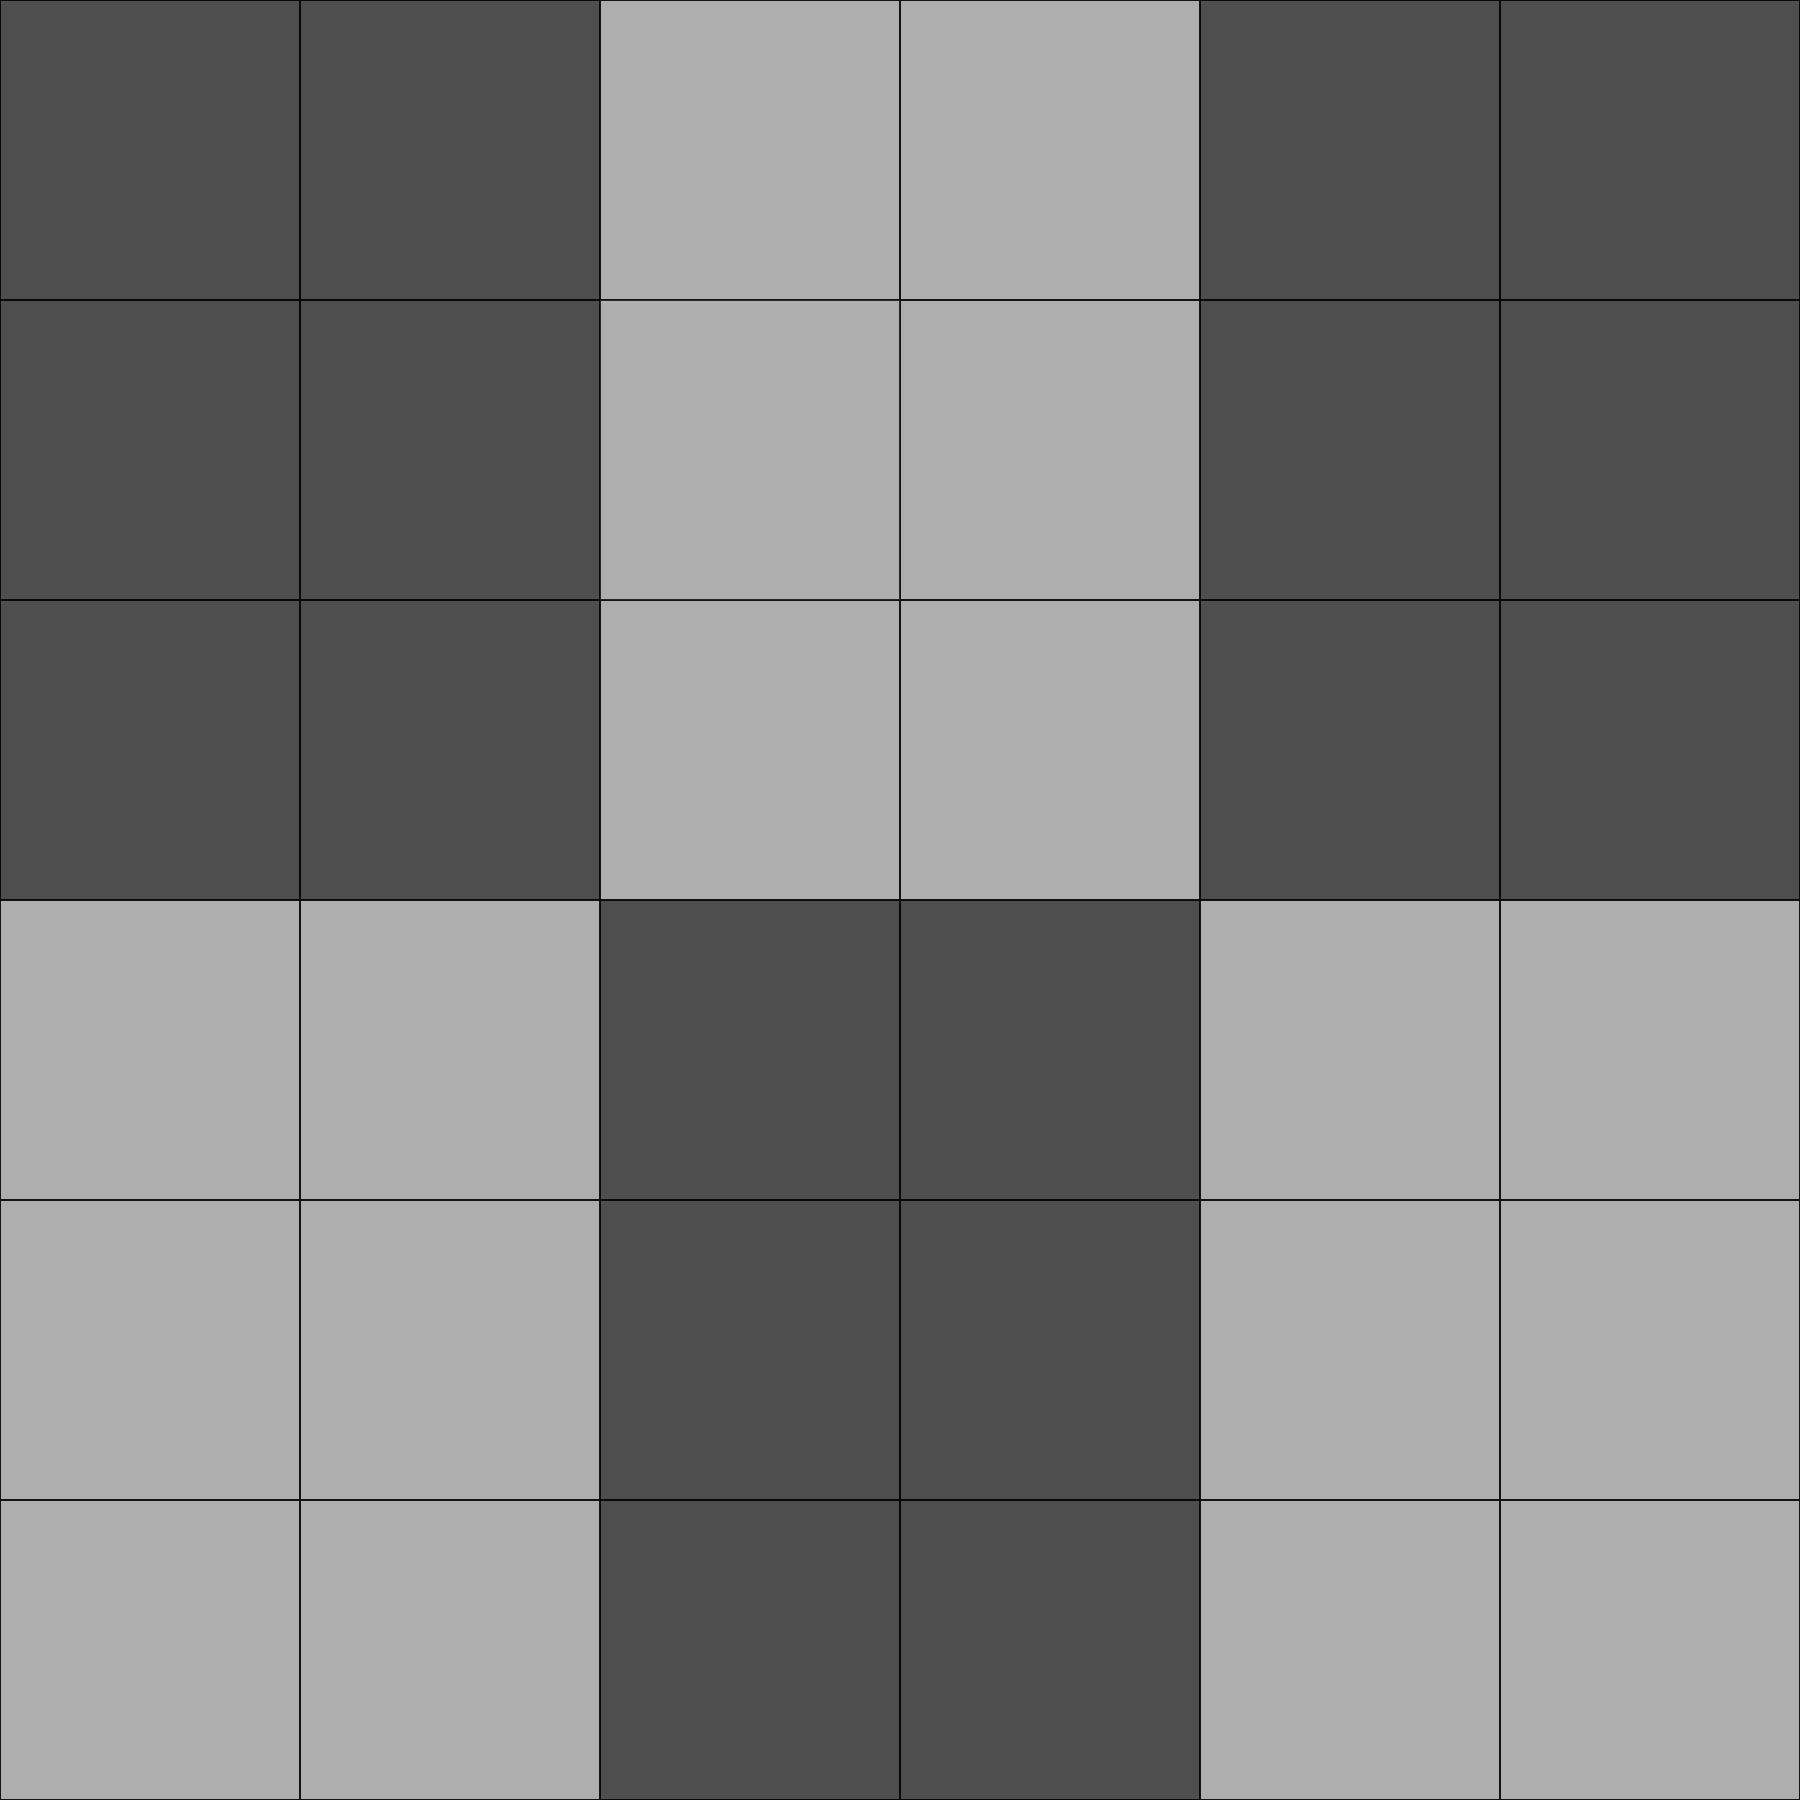
\includegraphics[height=0.7\textwidth]{pictures/2-1.png}
					\end{minipage}
					\begin{minipage}[t]{0.32\textwidth}
						\centering
						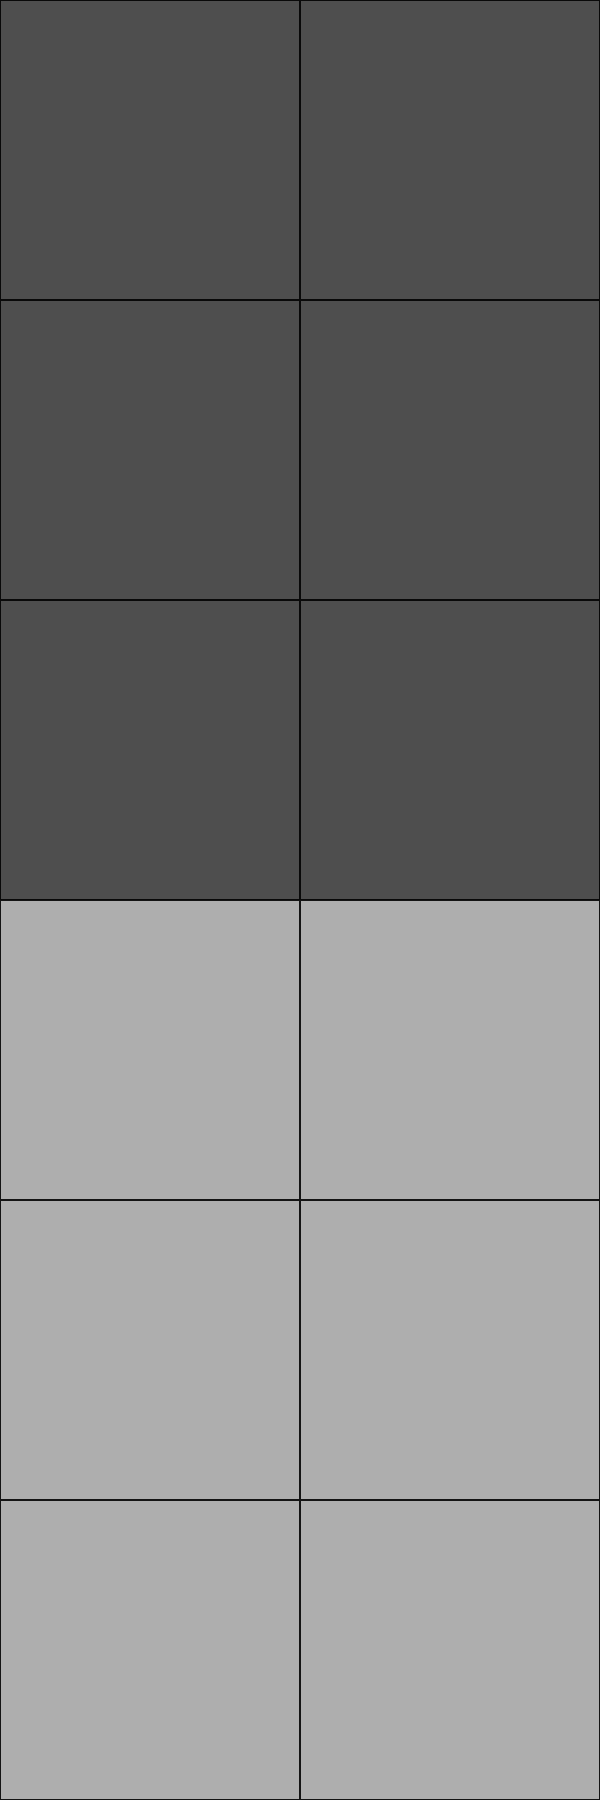
\includegraphics[height=0.7\textwidth]{pictures/2-2.png}
					\end{minipage}
					\begin{minipage}[t]{0.32\textwidth}
						\centering
						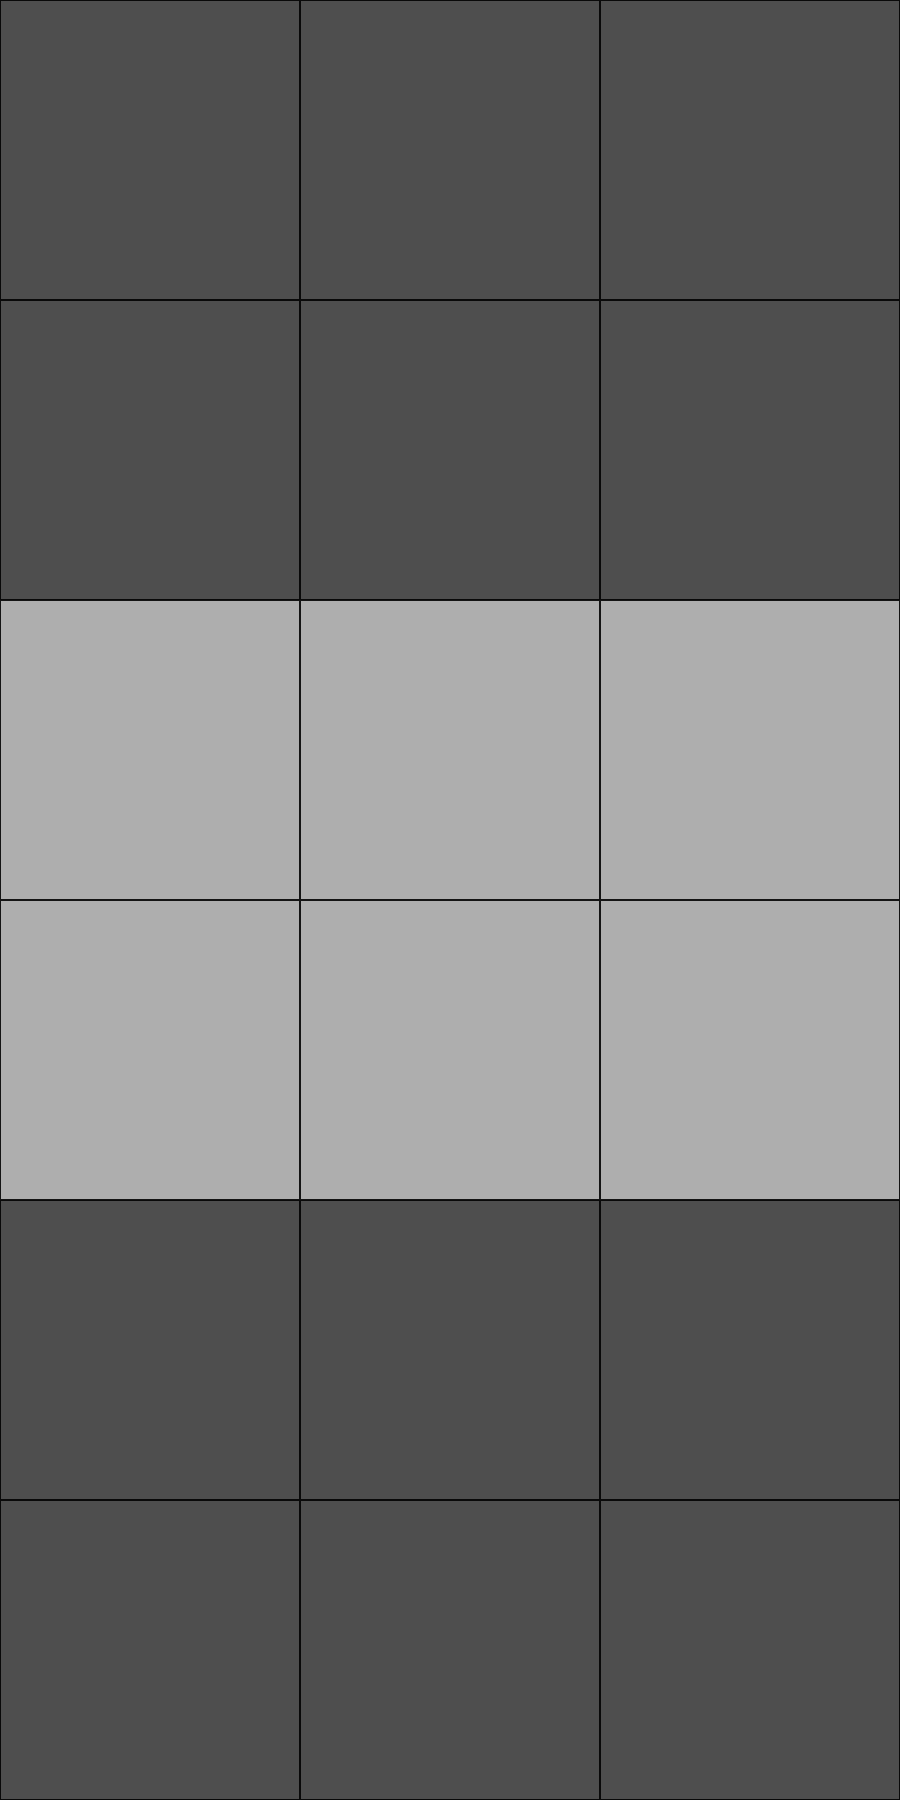
\includegraphics[height=0.7\textwidth]{pictures/2-3.png}
					\end{minipage}
				\end{figure}
				\begin{figure}[htbp]
					\centering
					\begin{minipage}[t]{0.32\textwidth}
						\centering
						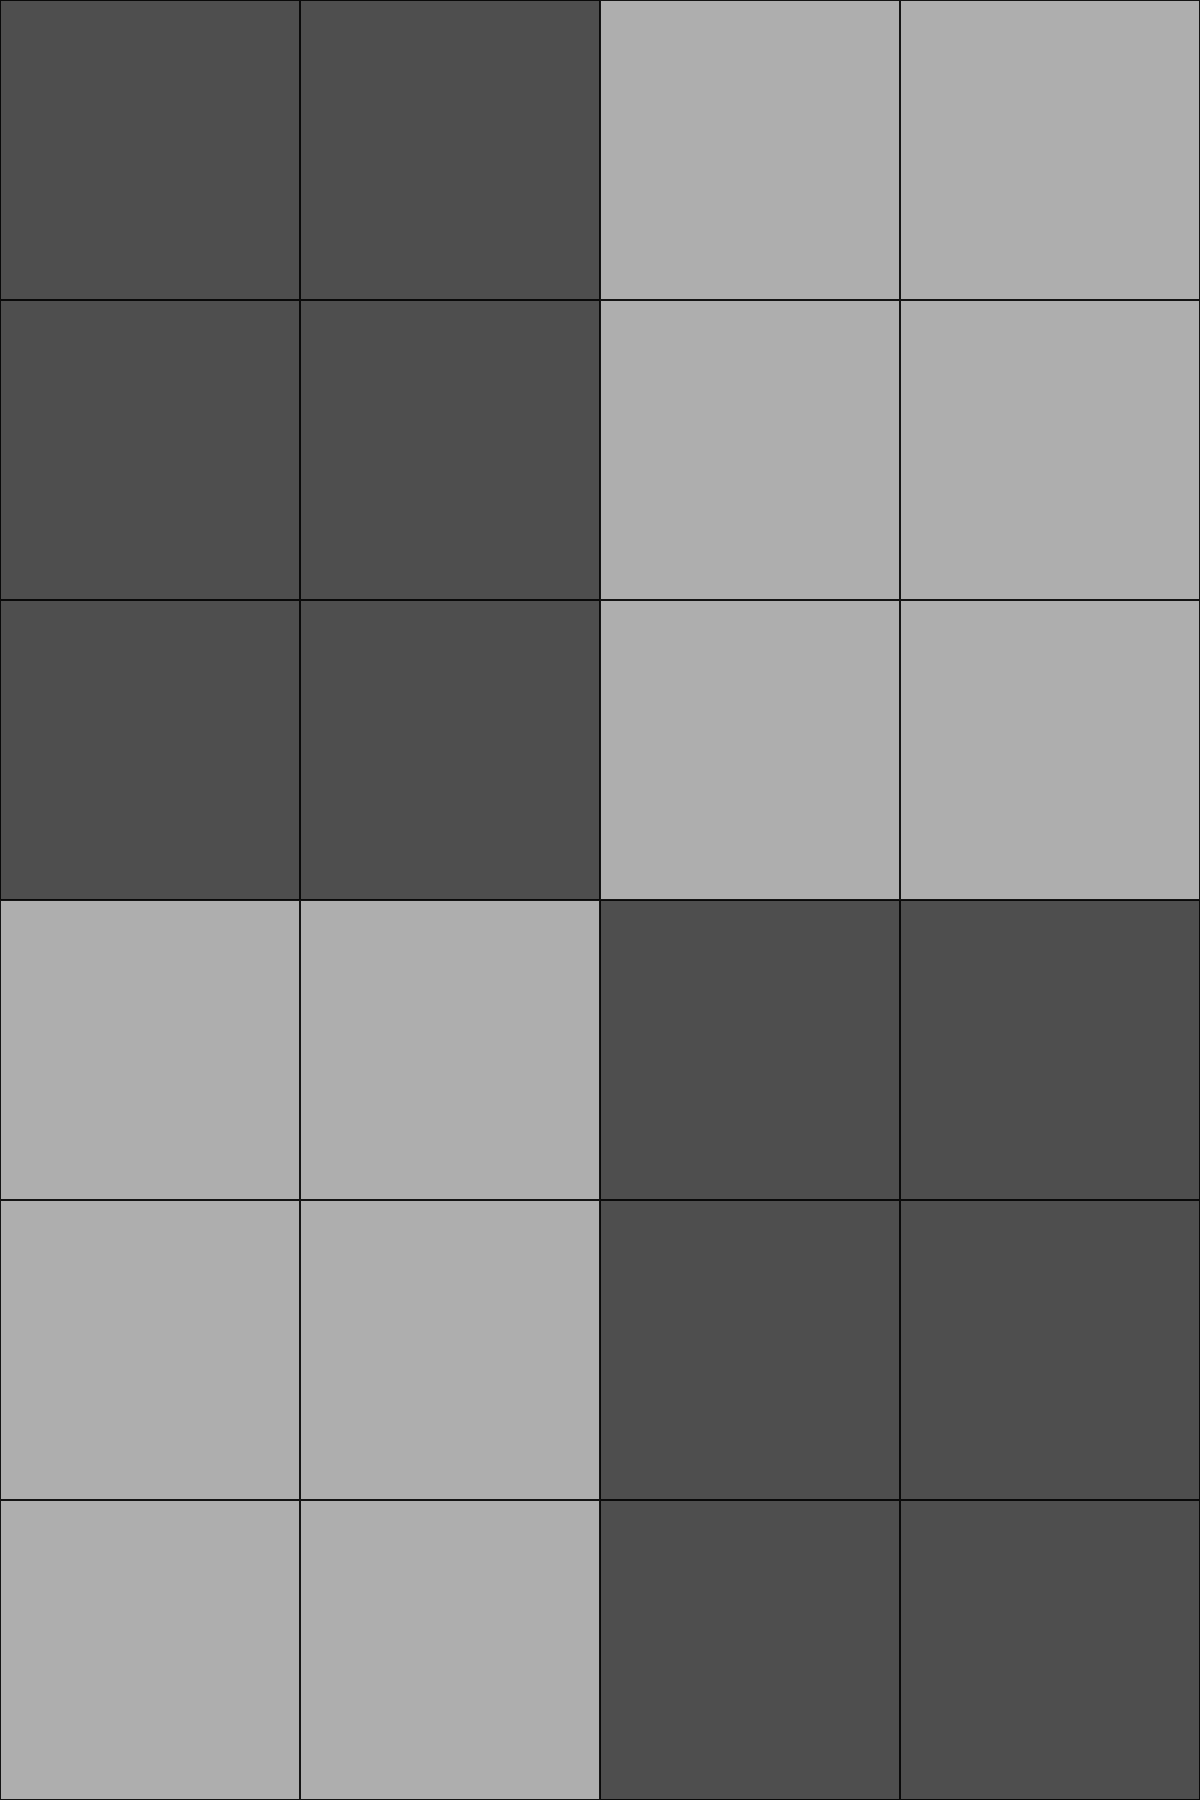
\includegraphics[height=0.7\textwidth]{pictures/2-4.png}
					\end{minipage}
					\begin{minipage}[t]{0.32\textwidth}
						\centering
						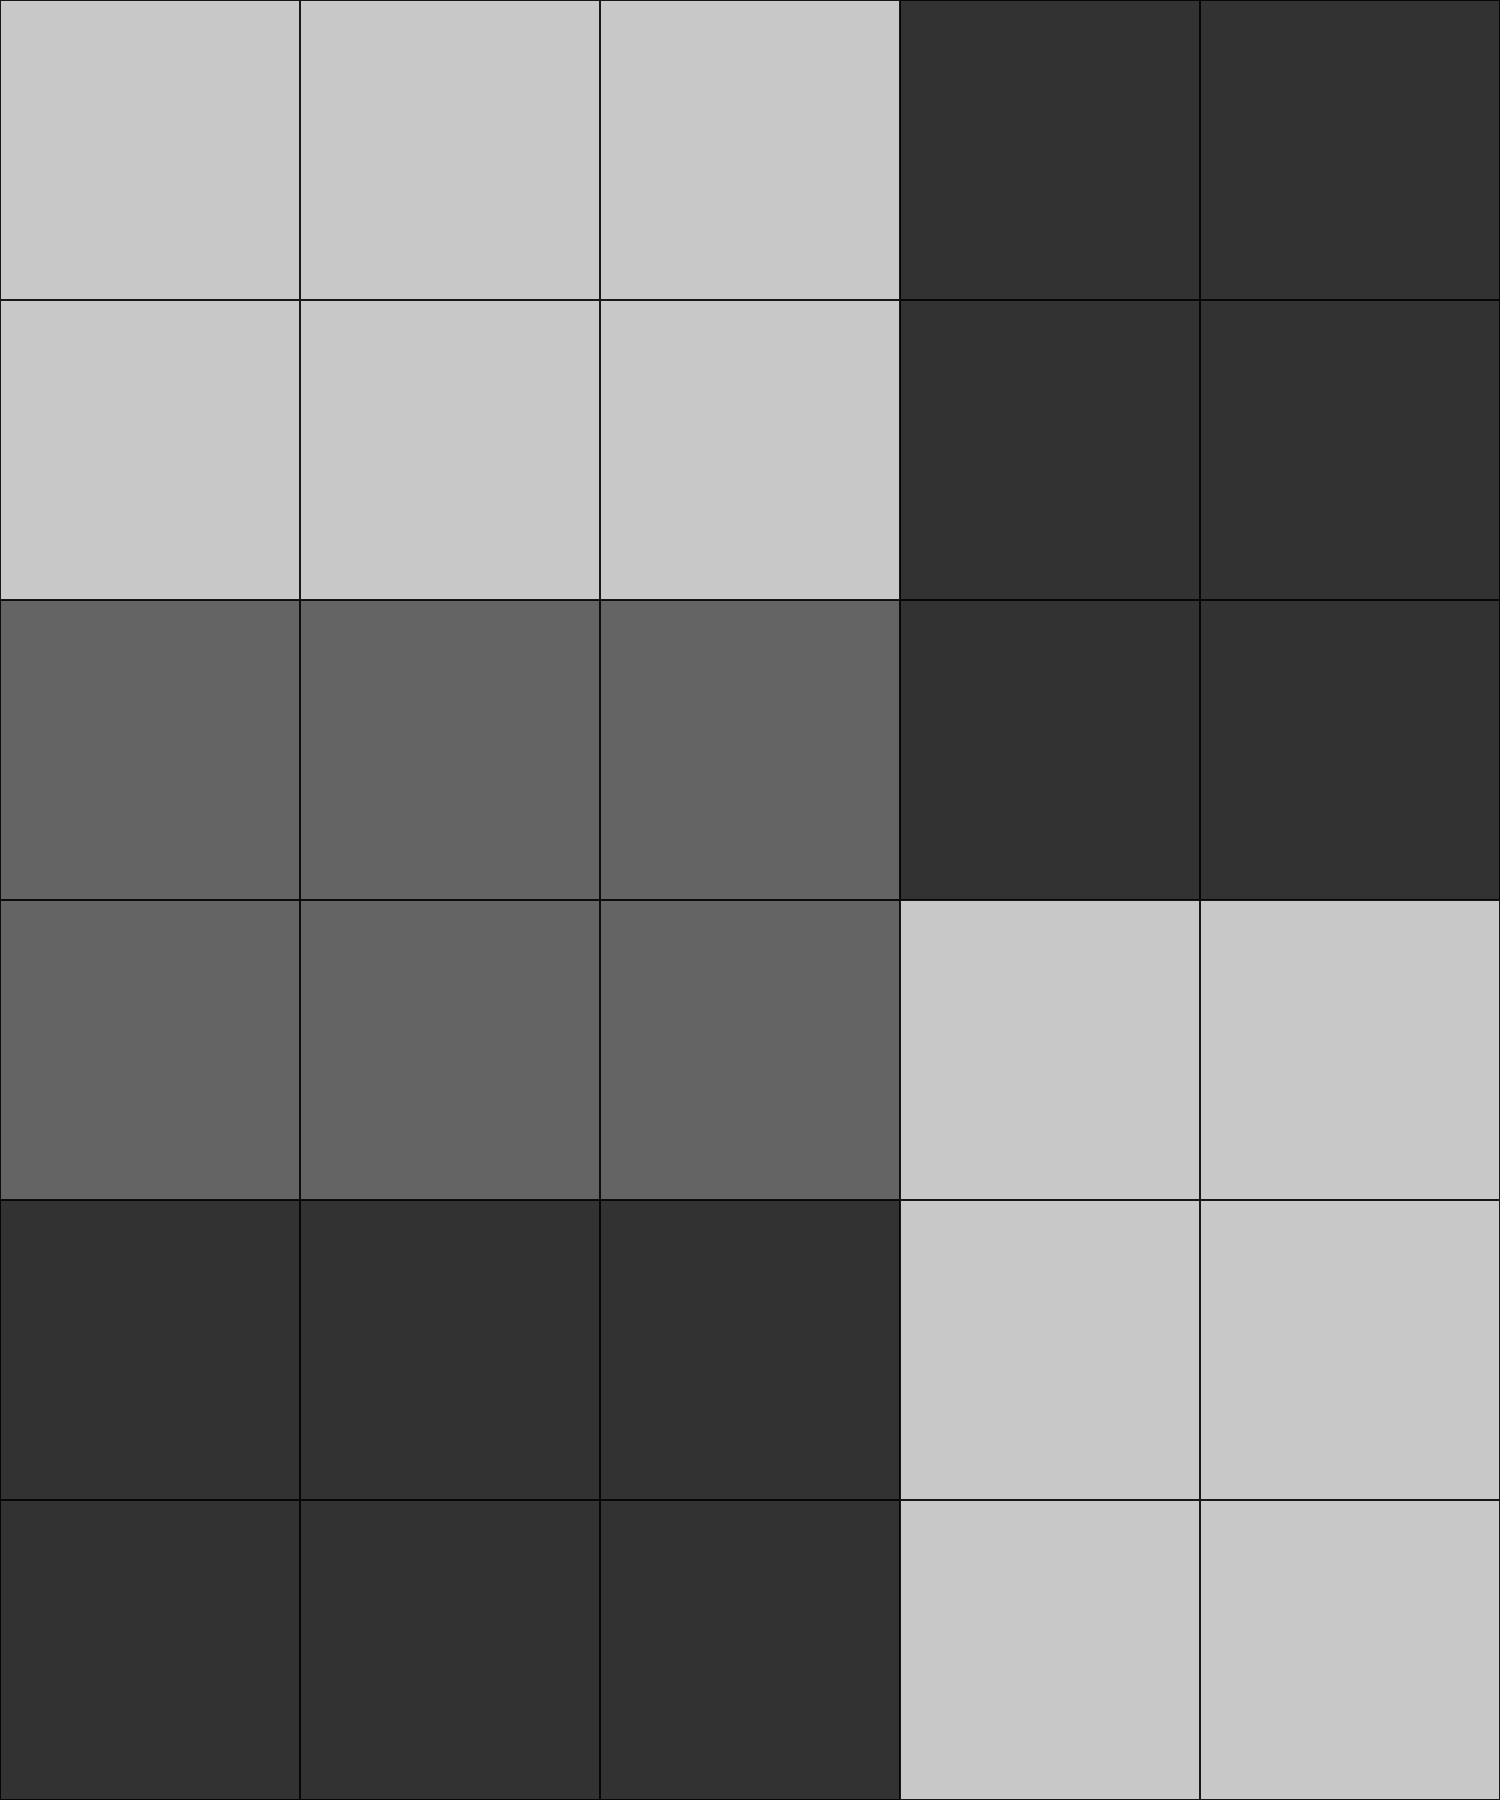
\includegraphics[height=0.7\textwidth]{pictures/2-5.png}
					\end{minipage}
					\begin{minipage}[t]{0.32\textwidth}
						\centering
						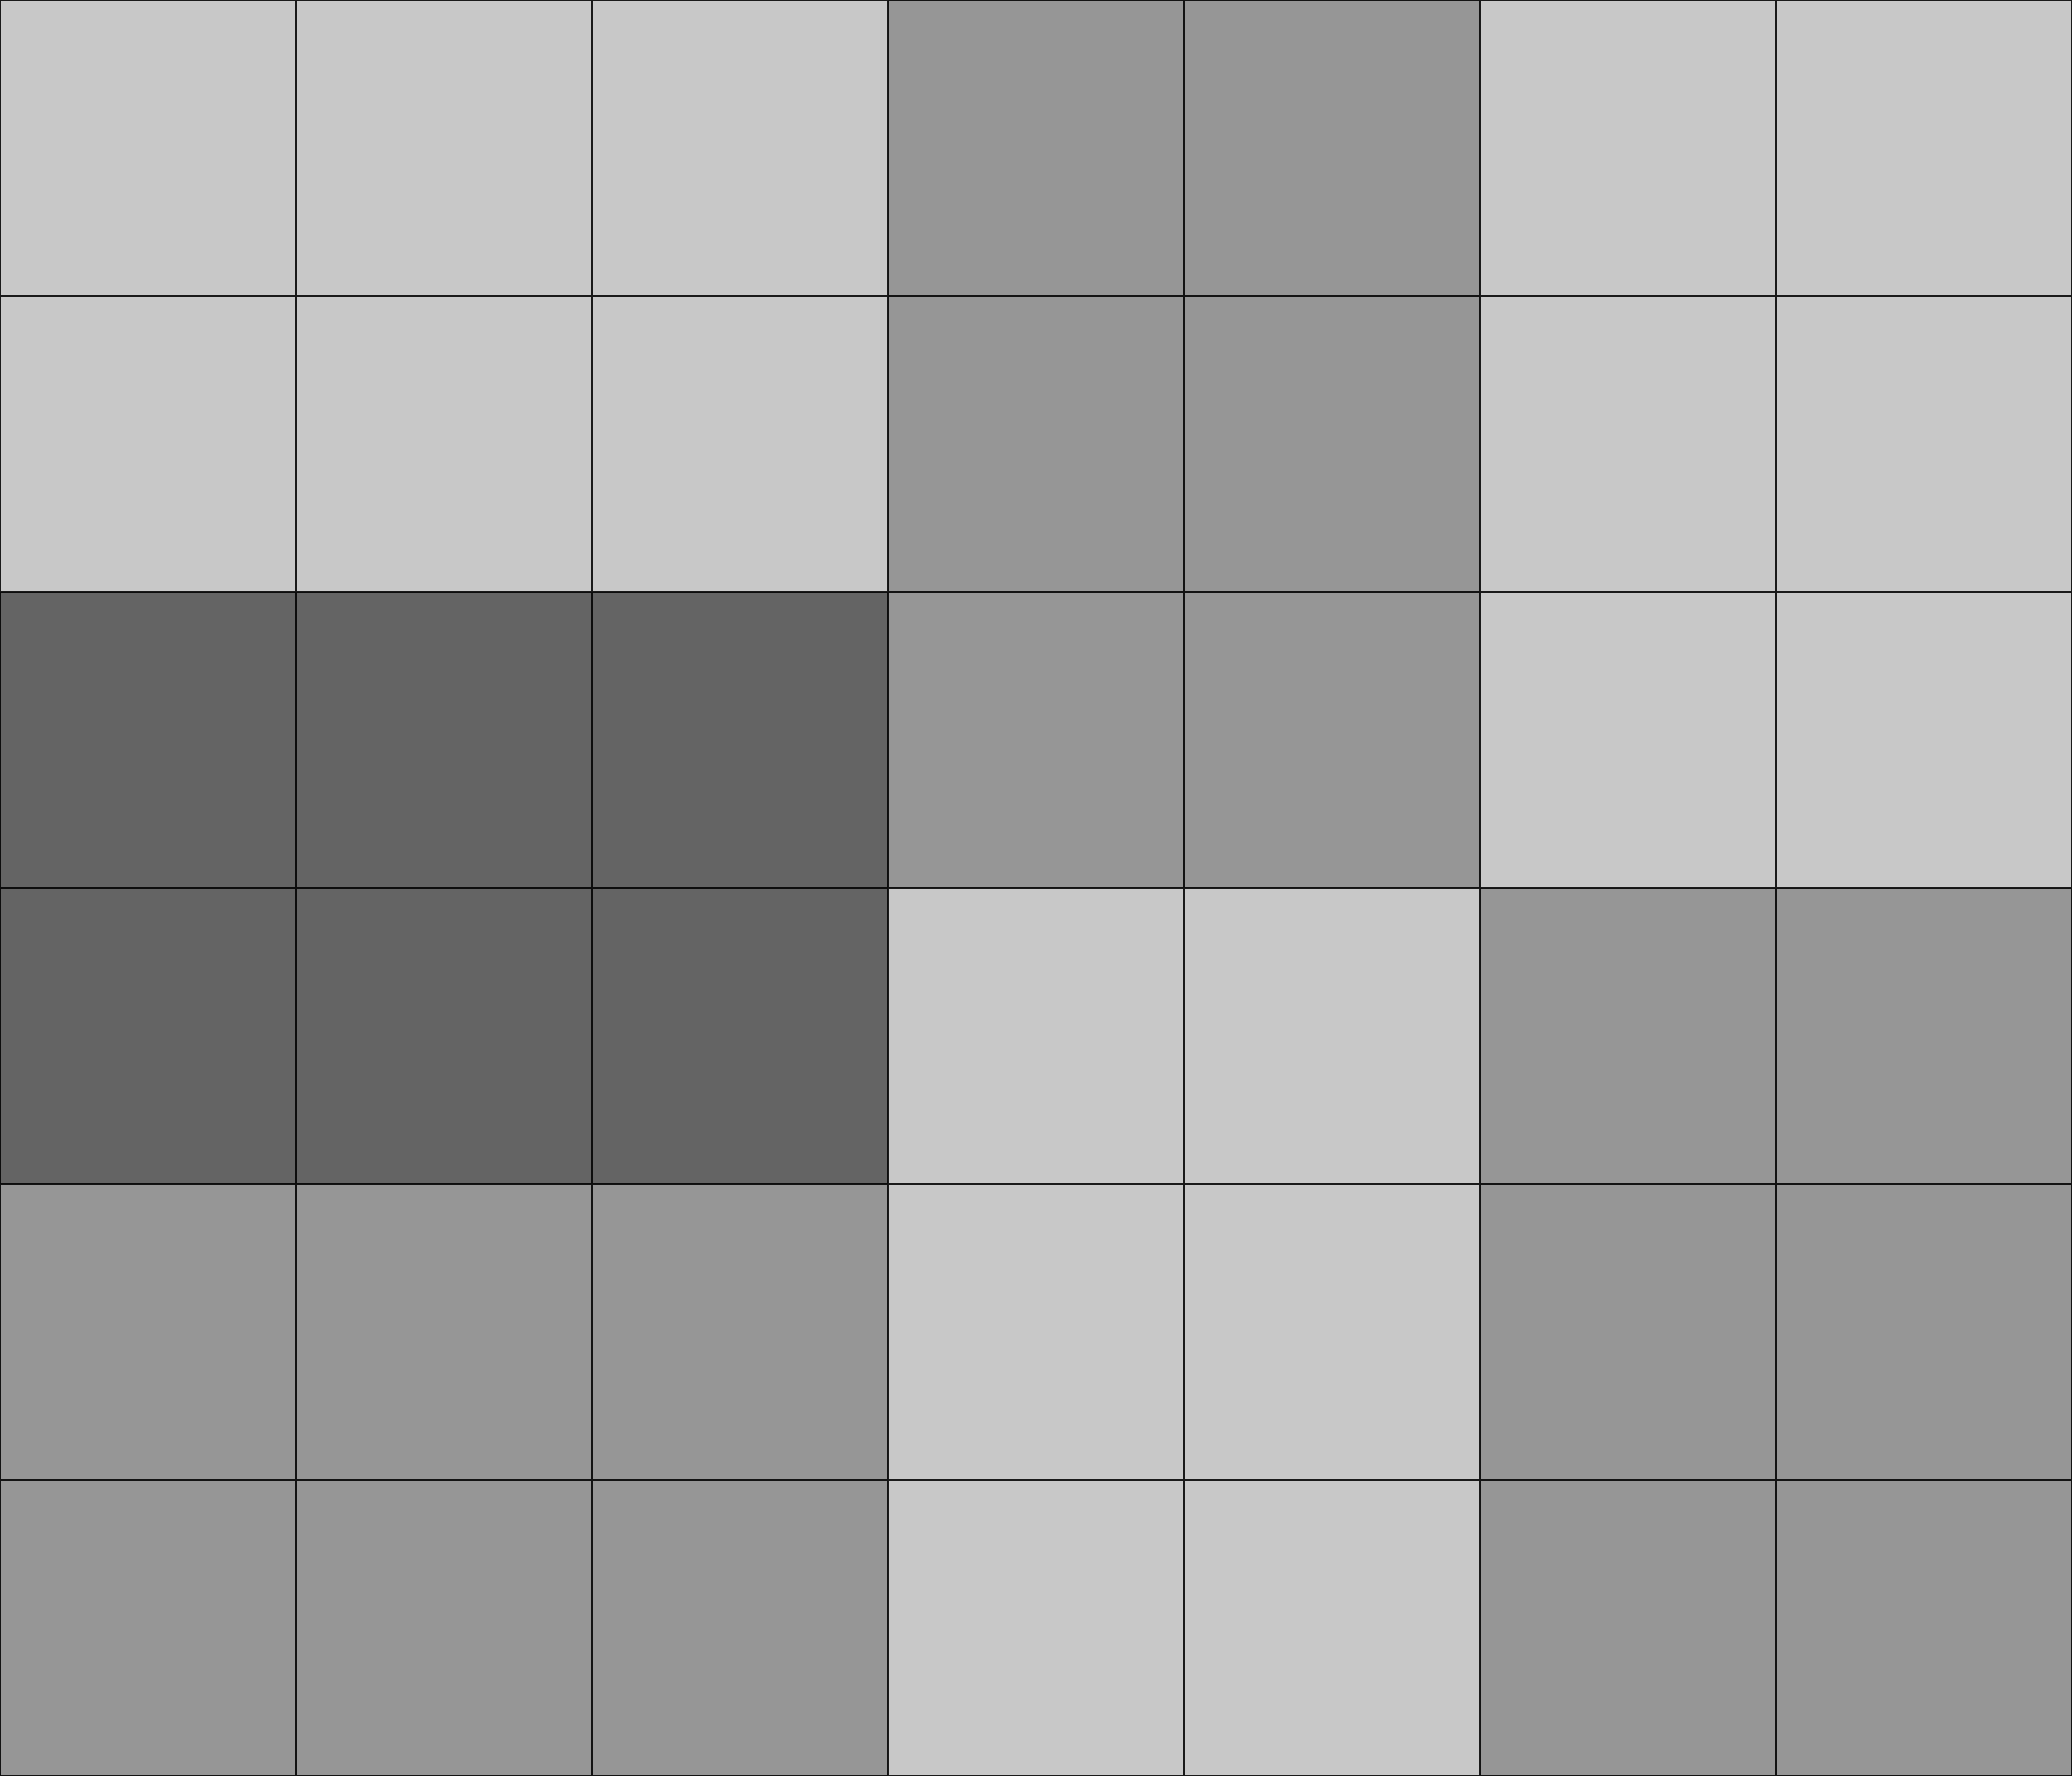
\includegraphics[height=0.7\textwidth]{pictures/2-6.png}
					\end{minipage}
				\end{figure}

				\centering{六种情况对应的方案}
			\end{frame}
			\begin{frame}\frametitle{$r=4$时}
				由于$4\times6$的可以填满,所以只需要讨论$c\bmod6$的值,找到一种填的方法使留空的格子数小于6\\
				若$c\bmod6=0$,则直接放满就行\\
				若$c\bmod6=1$,就不放,反正只留了4个空\\
				若$c\bmod6=2$,放一个$3\times2$\\
				若$c\bmod6=3$,放两个$2\times3$\\
				若$c\bmod6=4$,放两个$2\times3$\\
				若$c\bmod6=5$,放两个$2\times3$和一个$3\times2$\\
			\end{frame}
			\begin{frame}\frametitle{良心插图}
				\begin{figure}[htbp]
					\centering
					\begin{minipage}[t]{0.48\textwidth}
						\centering
						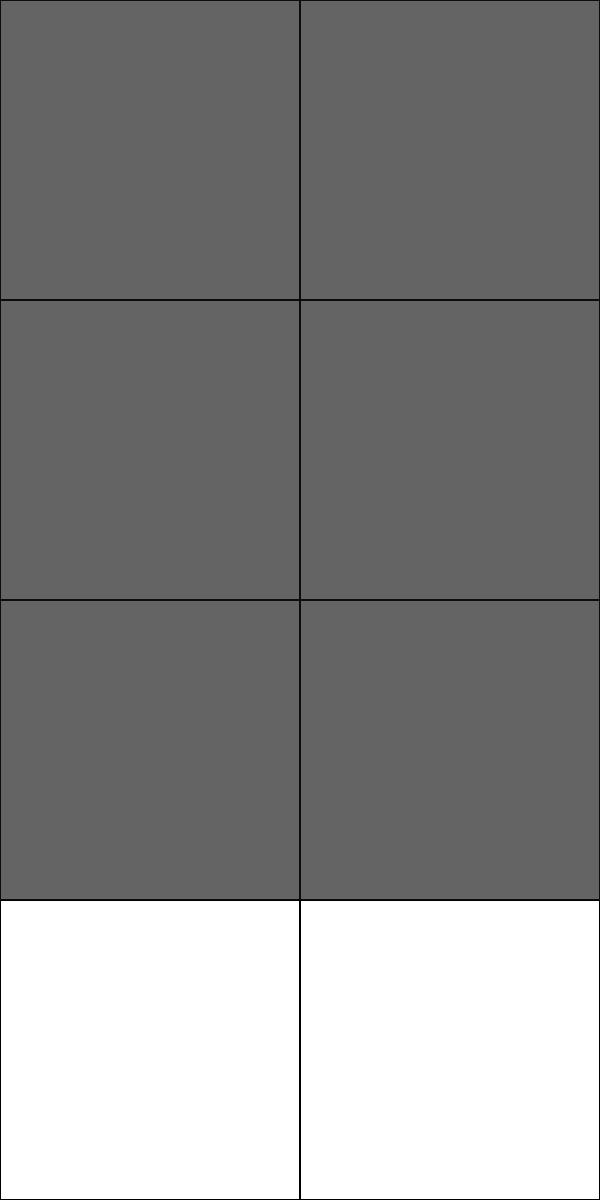
\includegraphics[height=0.5\textwidth]{pictures/3-1.png}
					\end{minipage}
					\begin{minipage}[t]{0.48\textwidth}
						\centering
						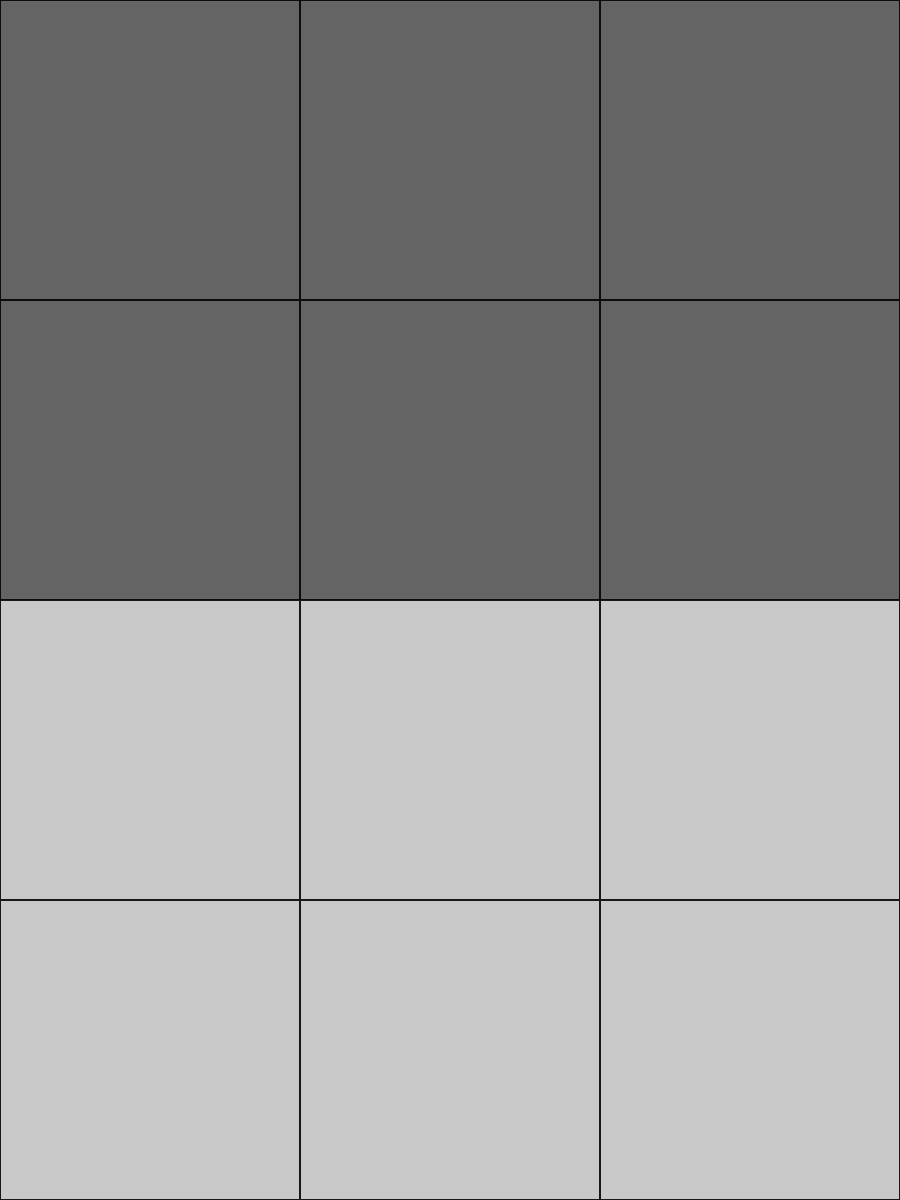
\includegraphics[height=0.5\textwidth]{pictures/3-2.png}
					\end{minipage}
				\end{figure}
				\begin{figure}[htbp]
					\centering
					\begin{minipage}[t]{0.48\textwidth}
						\centering
						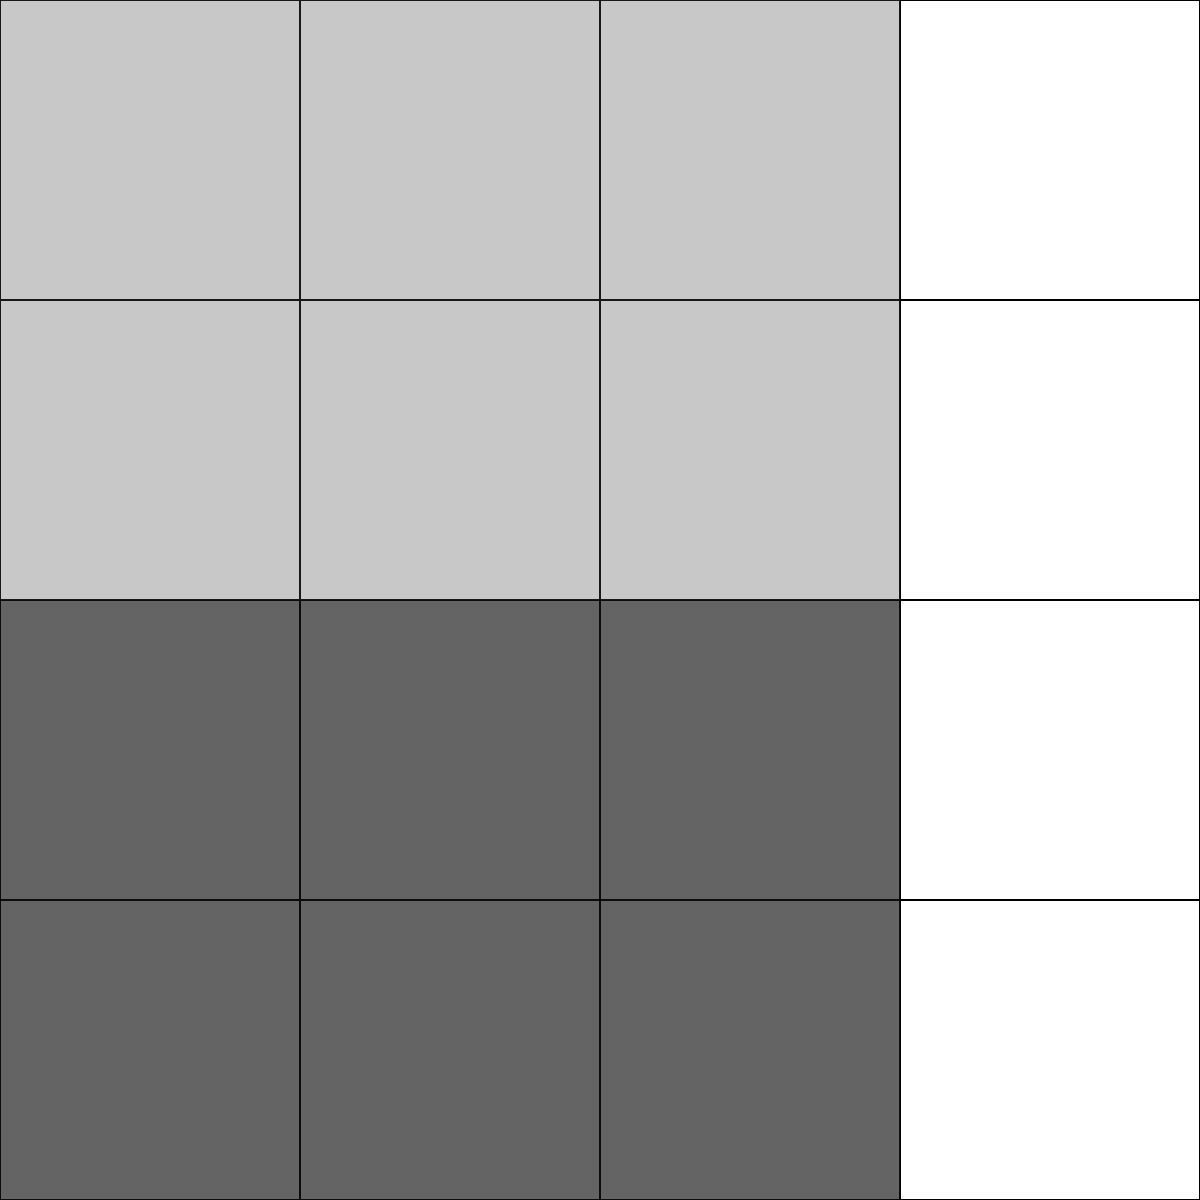
\includegraphics[height=0.5\textwidth]{pictures/3-3.png}
					\end{minipage}
					\begin{minipage}[t]{0.48\textwidth}
						\centering
						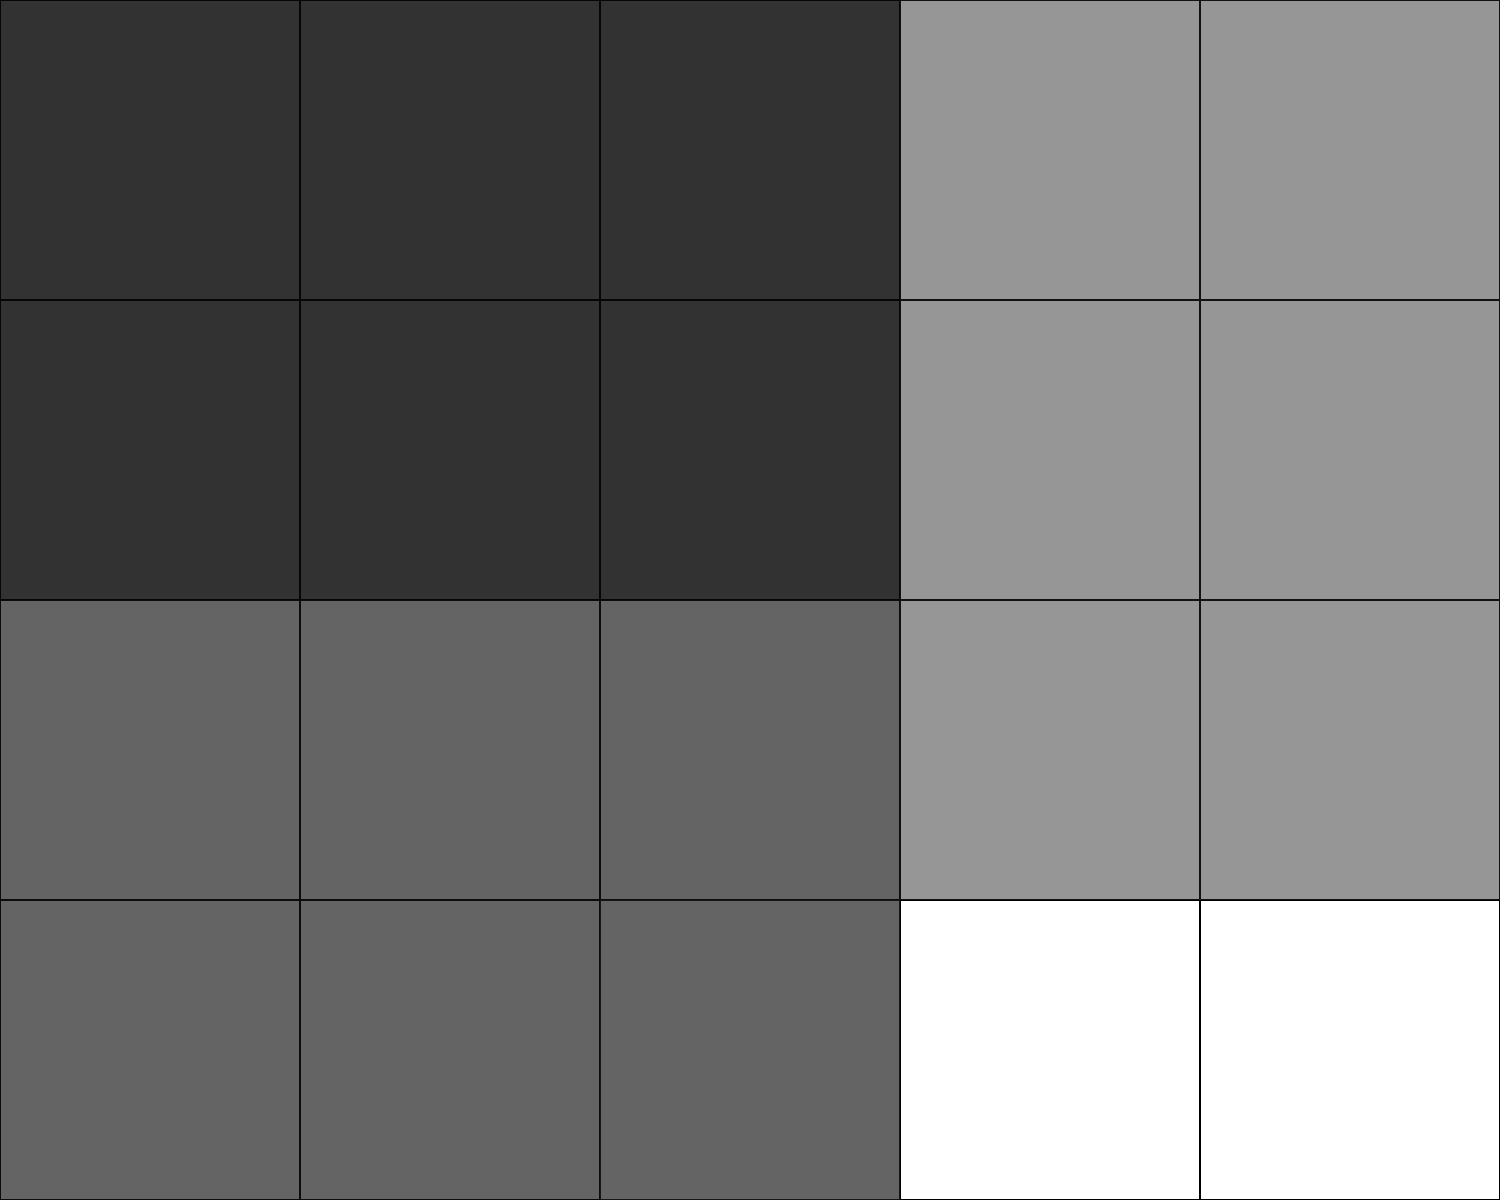
\includegraphics[height=0.5\textwidth]{pictures/3-4.png}
					\end{minipage}
				\end{figure}

				\centering{后四种情况对应的方案}
			\end{frame}
			\begin{frame}\frametitle{$r=5$时}
				由于$5\times6$的可以填满,所以只需要讨论$c\bmod6$的值,找到一种填的方法使留空的格子数小于6\\
				若$c\bmod6=0$,则直接放满就行\\
				若$c\bmod6=1$,就不放,反正只留了5个空\\
				若$c\bmod6=2$,放一个$3\times2$\\
				若$c\bmod6=3$,放两个$2\times3$\\
				若$c\bmod6=4$,放两个$2\times3$和一个$3\times2$\\
				若$c\bmod6=5$,像风车一样放两个$2\times3$和两个$3\times2$,中间留空一格\\
			\end{frame}
			\begin{frame}\frametitle{良心插图}
				\begin{figure}[htbp]
					\centering
					\begin{minipage}[t]{0.48\textwidth}
						\centering
						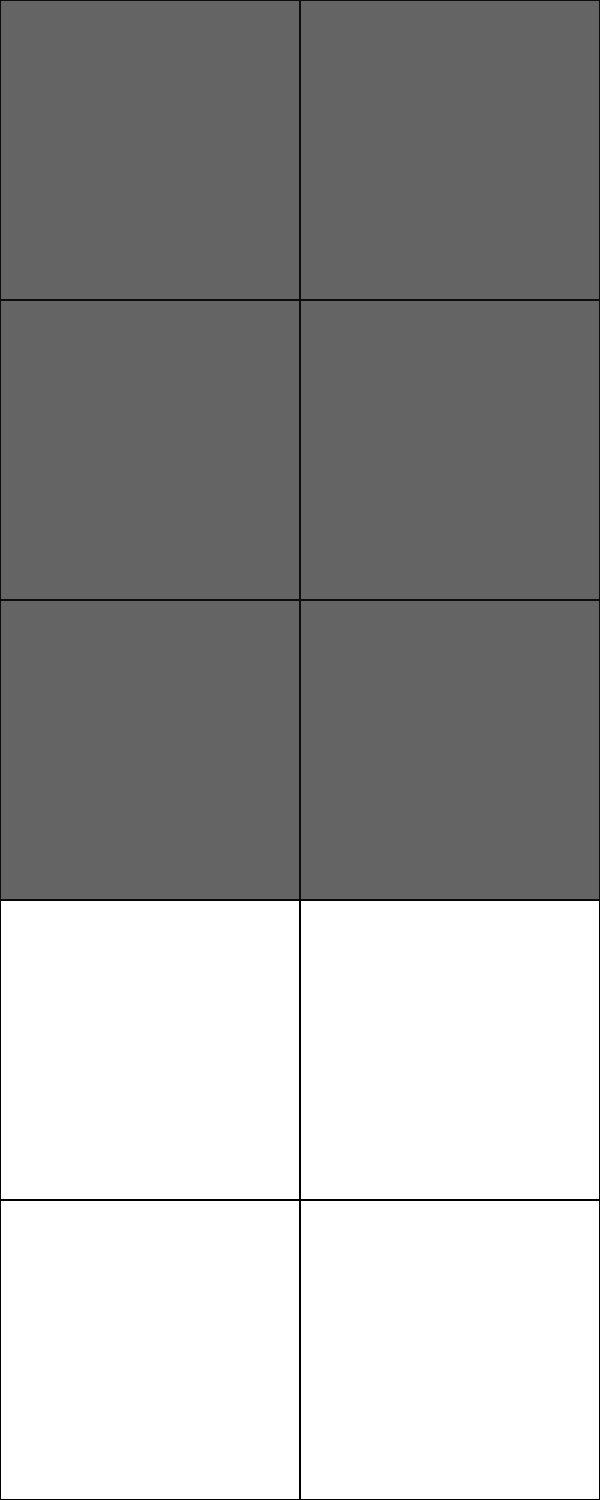
\includegraphics[height=0.5\textwidth]{pictures/4-1.png}
					\end{minipage}
					\begin{minipage}[t]{0.48\textwidth}
						\centering
						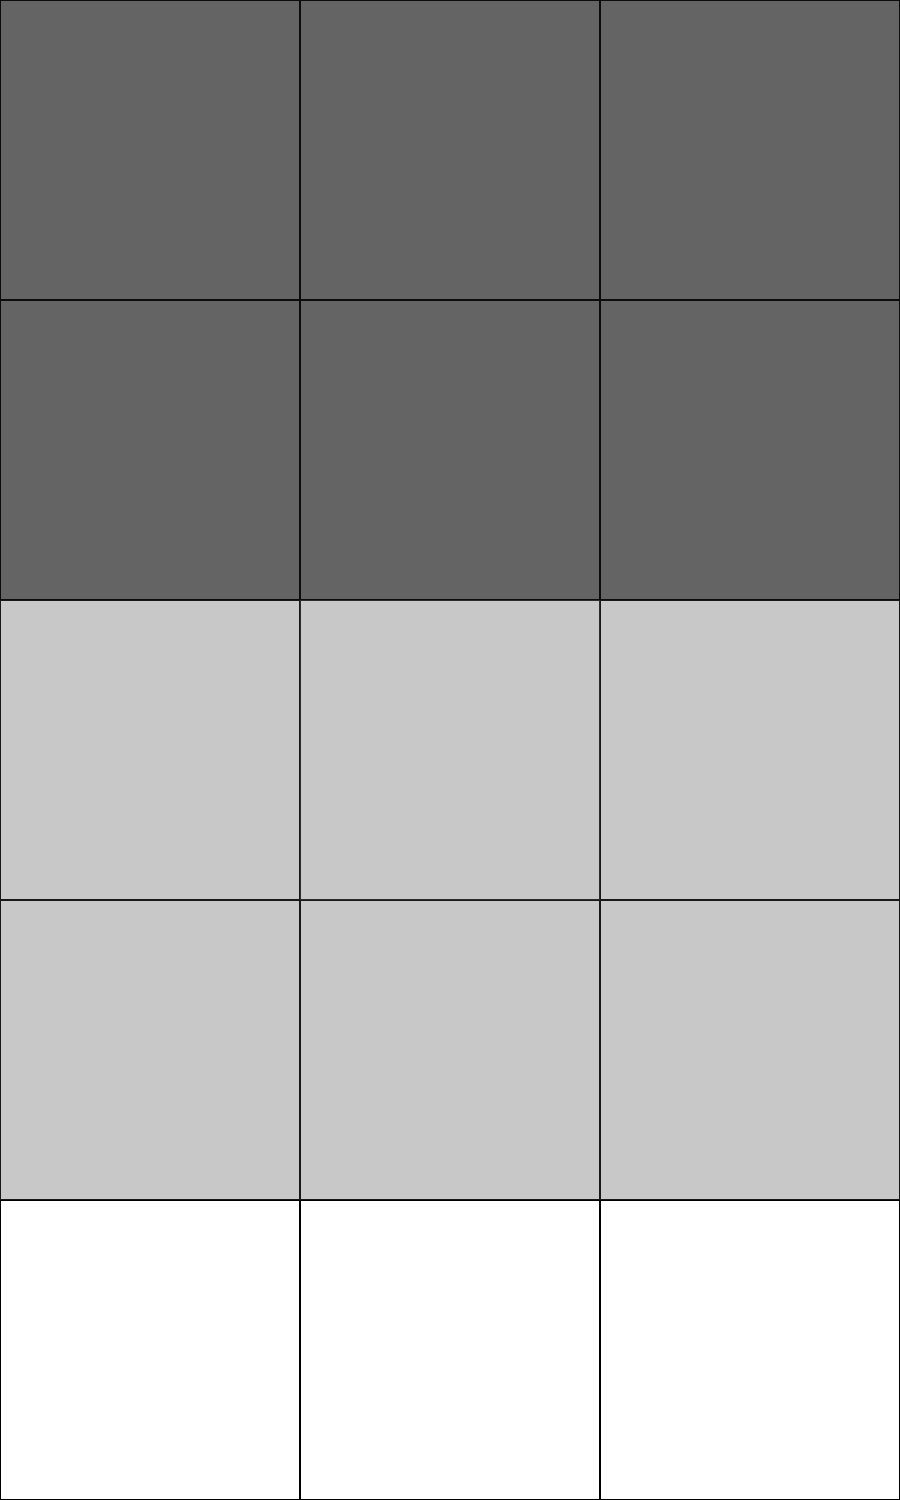
\includegraphics[height=0.5\textwidth]{pictures/4-2.png}
					\end{minipage}
				\end{figure}
				\begin{figure}[htbp]
					\centering
					\begin{minipage}[t]{0.48\textwidth}
						\centering
						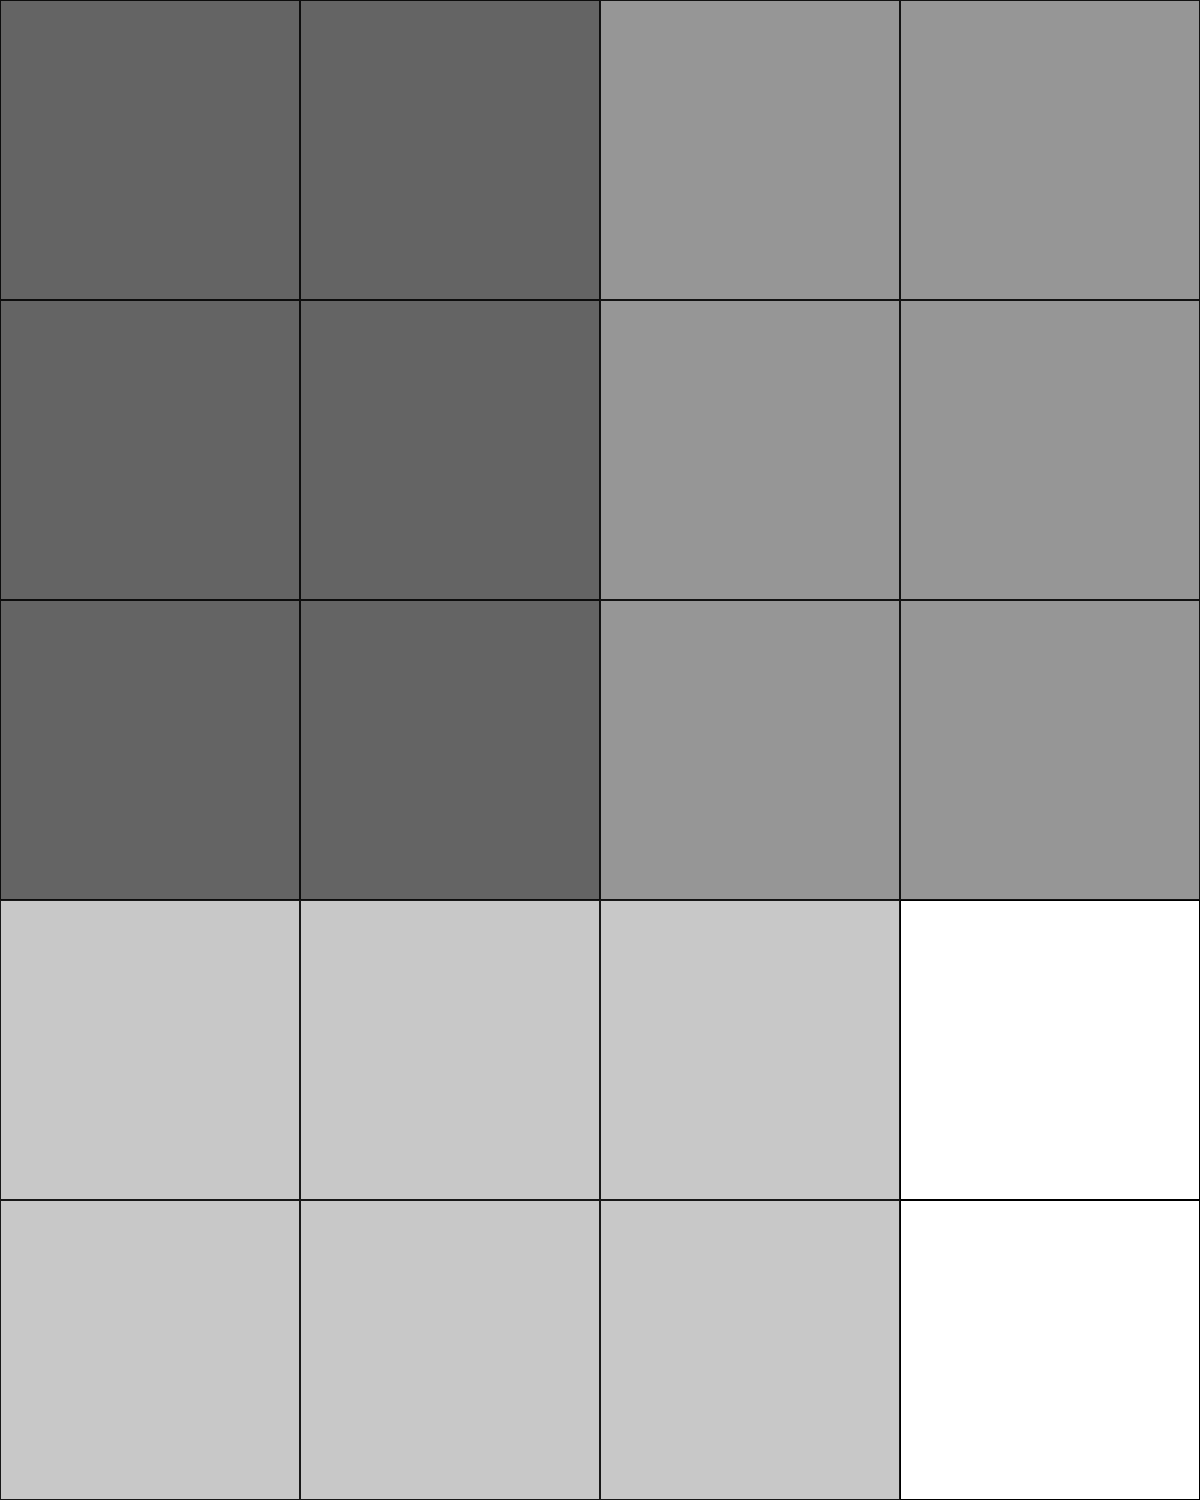
\includegraphics[height=0.5\textwidth]{pictures/4-3.png}
					\end{minipage}
					\begin{minipage}[t]{0.48\textwidth}
						\centering
						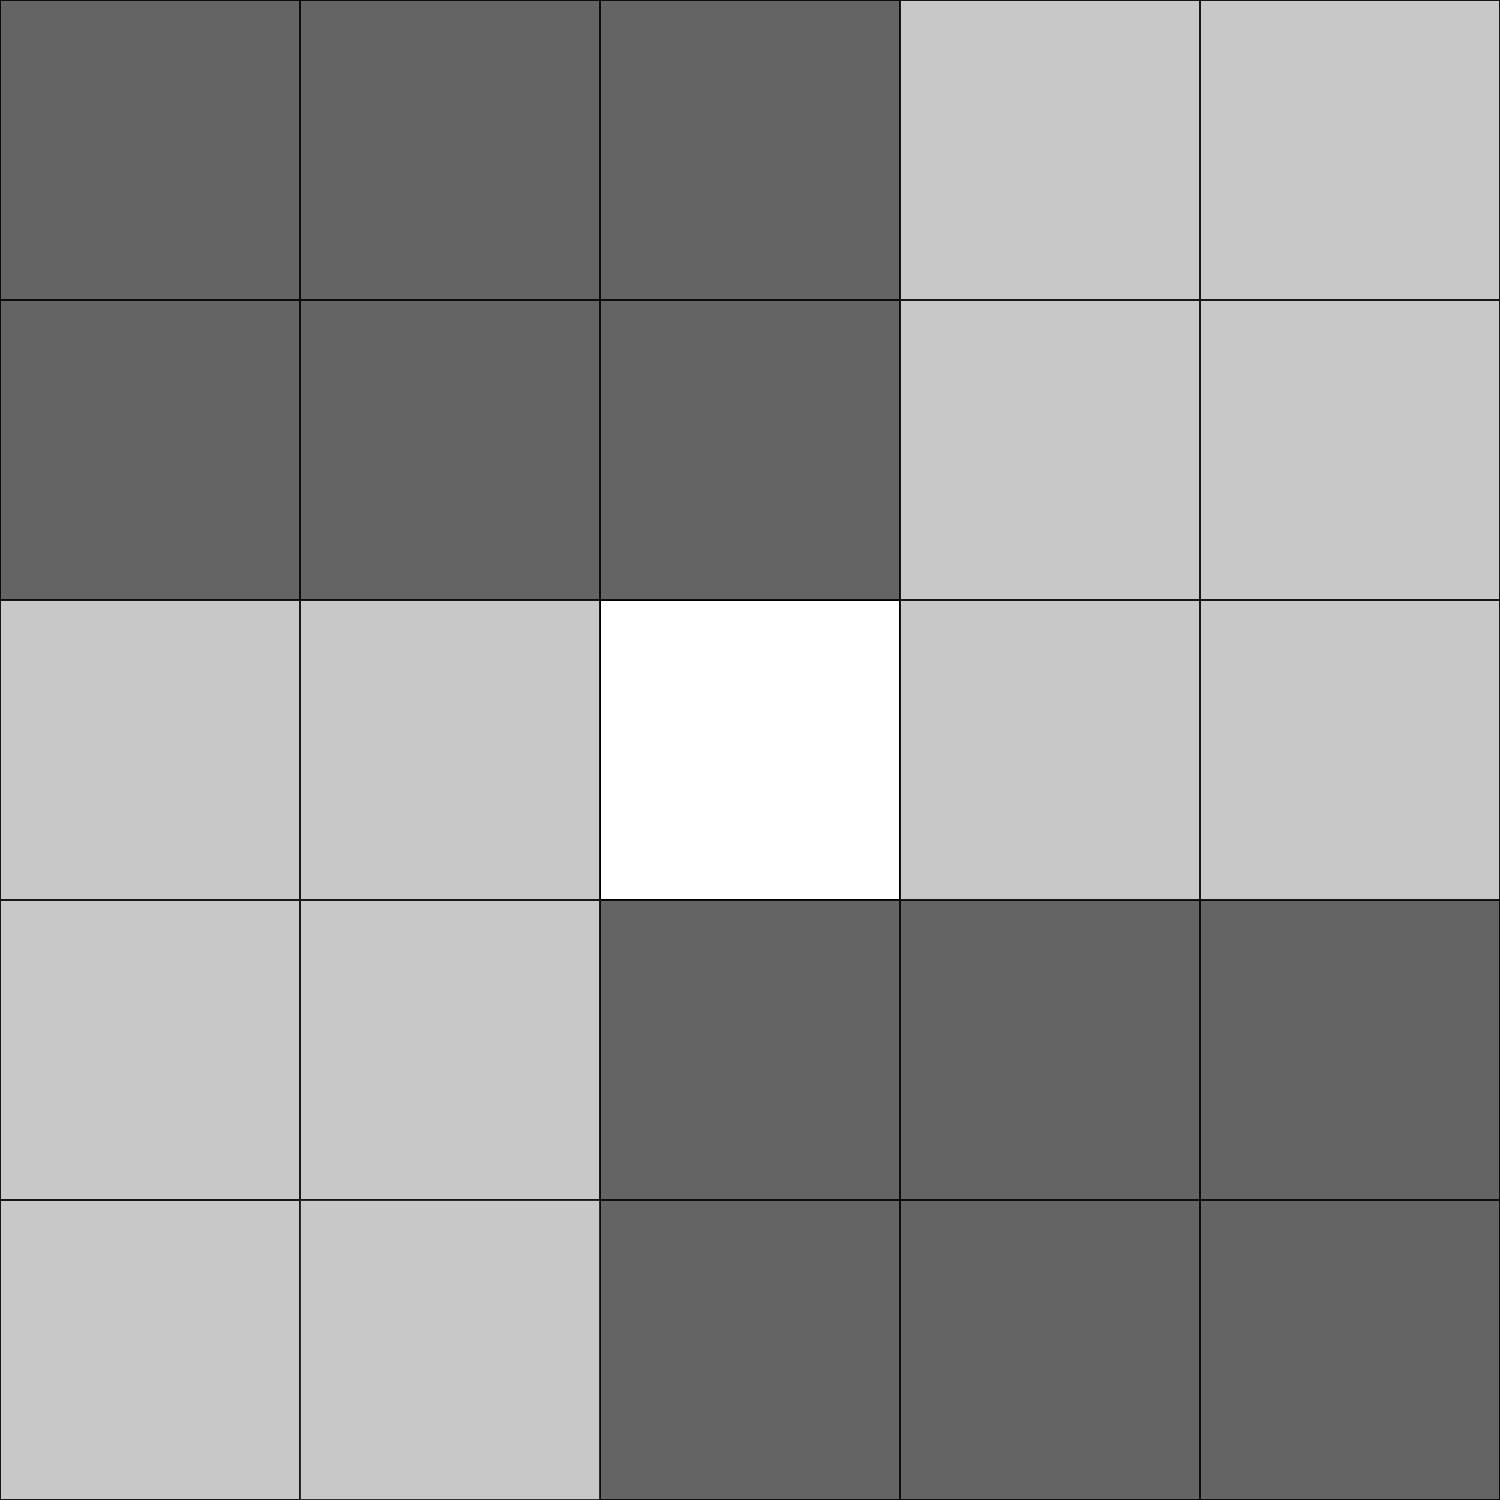
\includegraphics[height=0.5\textwidth]{pictures/4-4.png}
					\end{minipage}
				\end{figure}

				\centering{后四种情况对应的方案}
			\end{frame}
			\begin{frame}\frametitle{$r=7$时}
				由于$7\times6$的可以填满,所以只需要讨论$c\bmod6$的值,找到一种填的方法使留空的格子数小于6\\
				若$c\bmod6=0$,则直接放满就行\\
				若$c\bmod6=2$,放一个$6\times2$\\
				若$c\bmod6=3$,放一个$6\times3$\\
				若$c\bmod6=4$,放一个$6\times4$\\
				若$c\bmod6=5$,放一个$6\times5$\\
				若$c\bmod6=1$,则$c\ge7$,像风车一样放两个$3\times4$和两个$4\times3$就行\\
			\end{frame}
			\begin{frame}\frametitle{良心插图}
				\begin{figure}[htbp]
					\centering
					\begin{minipage}[t]{0.32\textwidth}
						\centering
						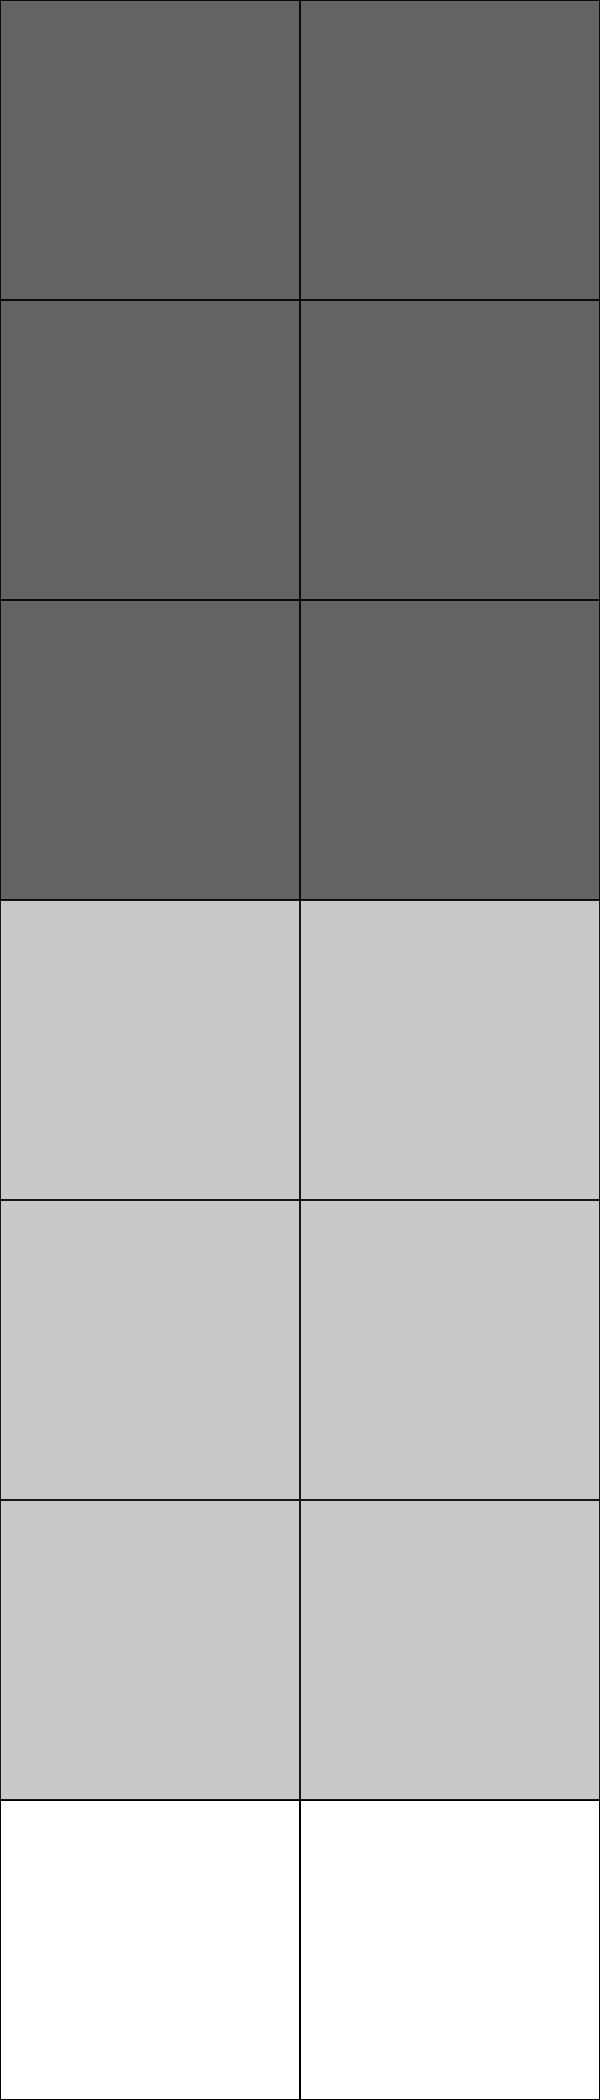
\includegraphics[height=0.68\textwidth]{pictures/5-1.png}
					\end{minipage}
					\begin{minipage}[t]{0.32\textwidth}
						\centering
						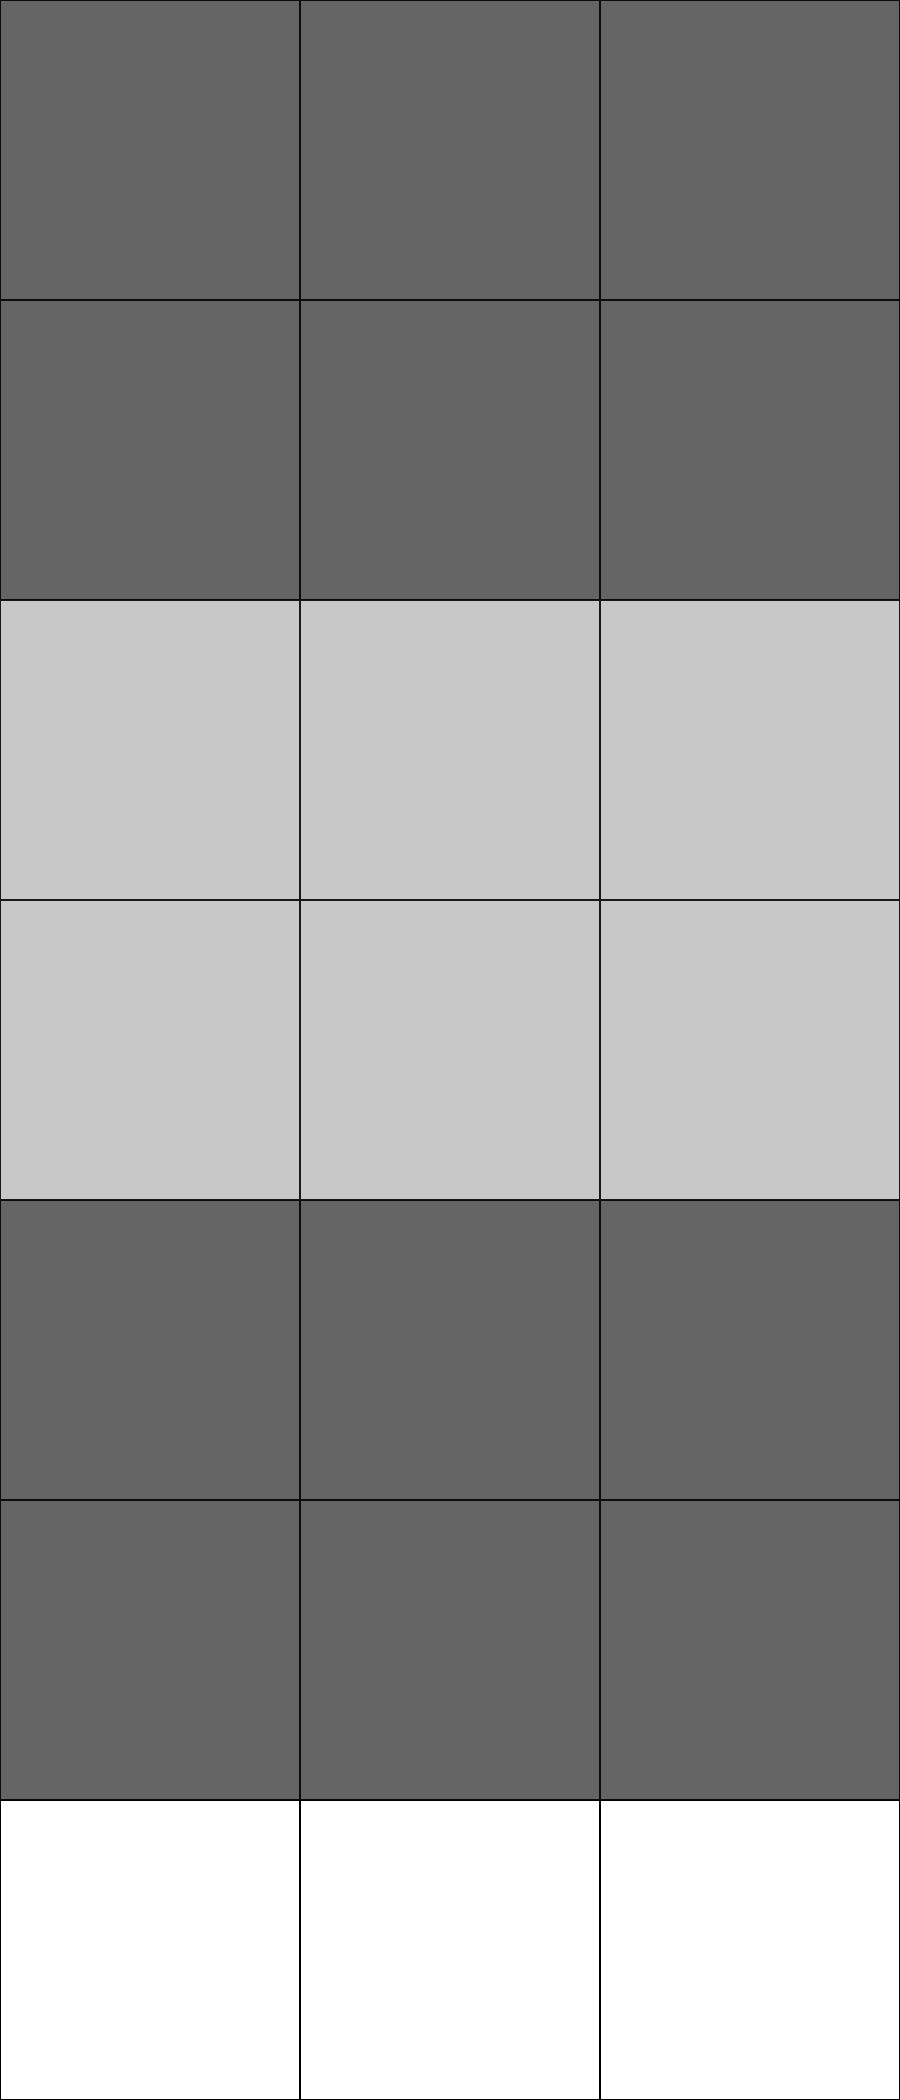
\includegraphics[height=0.68\textwidth]{pictures/5-2.png}
					\end{minipage}
					\begin{minipage}[t]{0.32\textwidth}
						\centering
						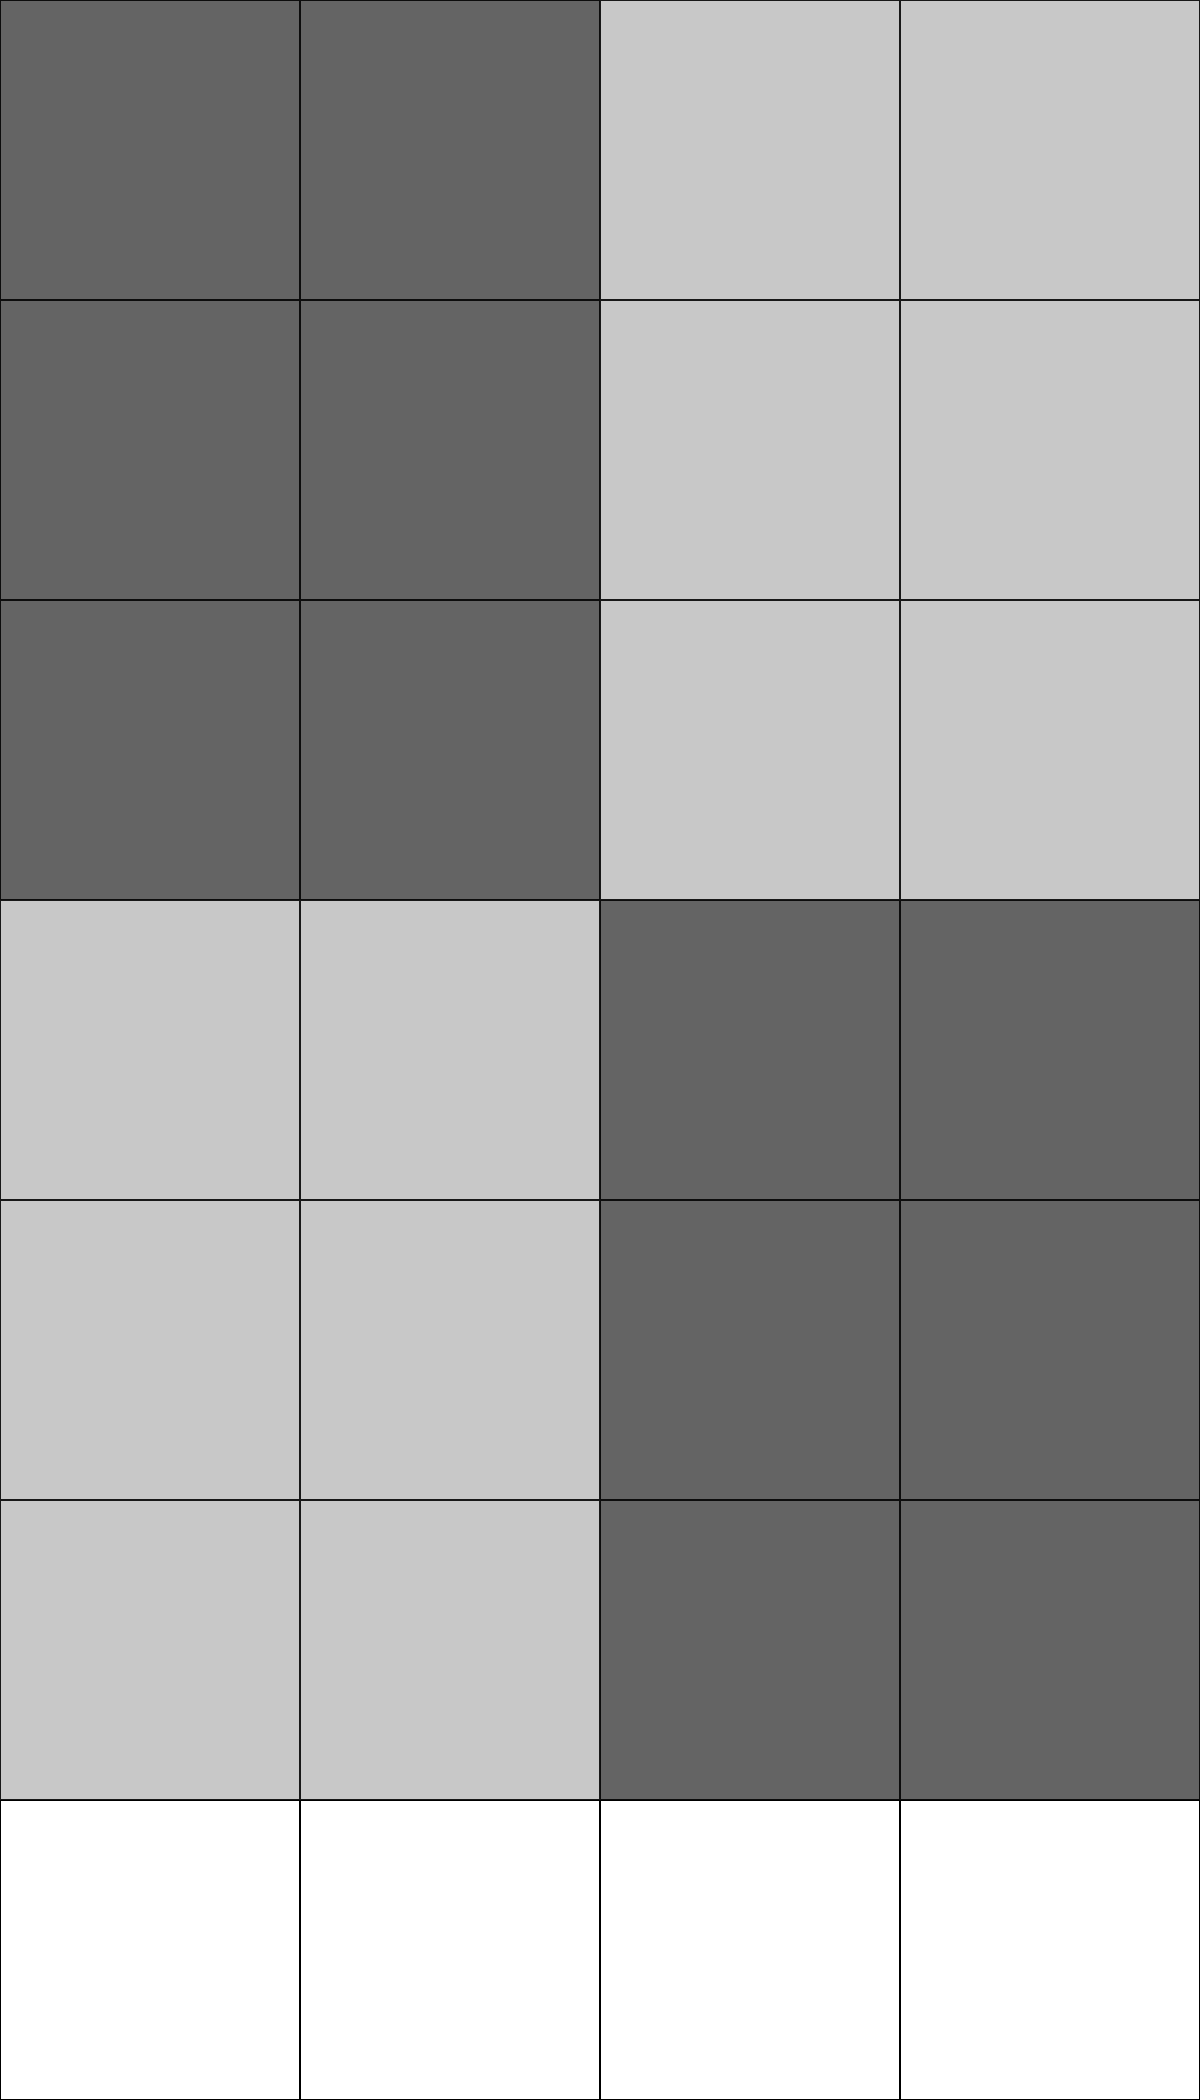
\includegraphics[height=0.68\textwidth]{pictures/5-3.png}
					\end{minipage}
				\end{figure}
				\begin{figure}[htbp]
					\centering
					\begin{minipage}[t]{0.48\textwidth}
						\centering
						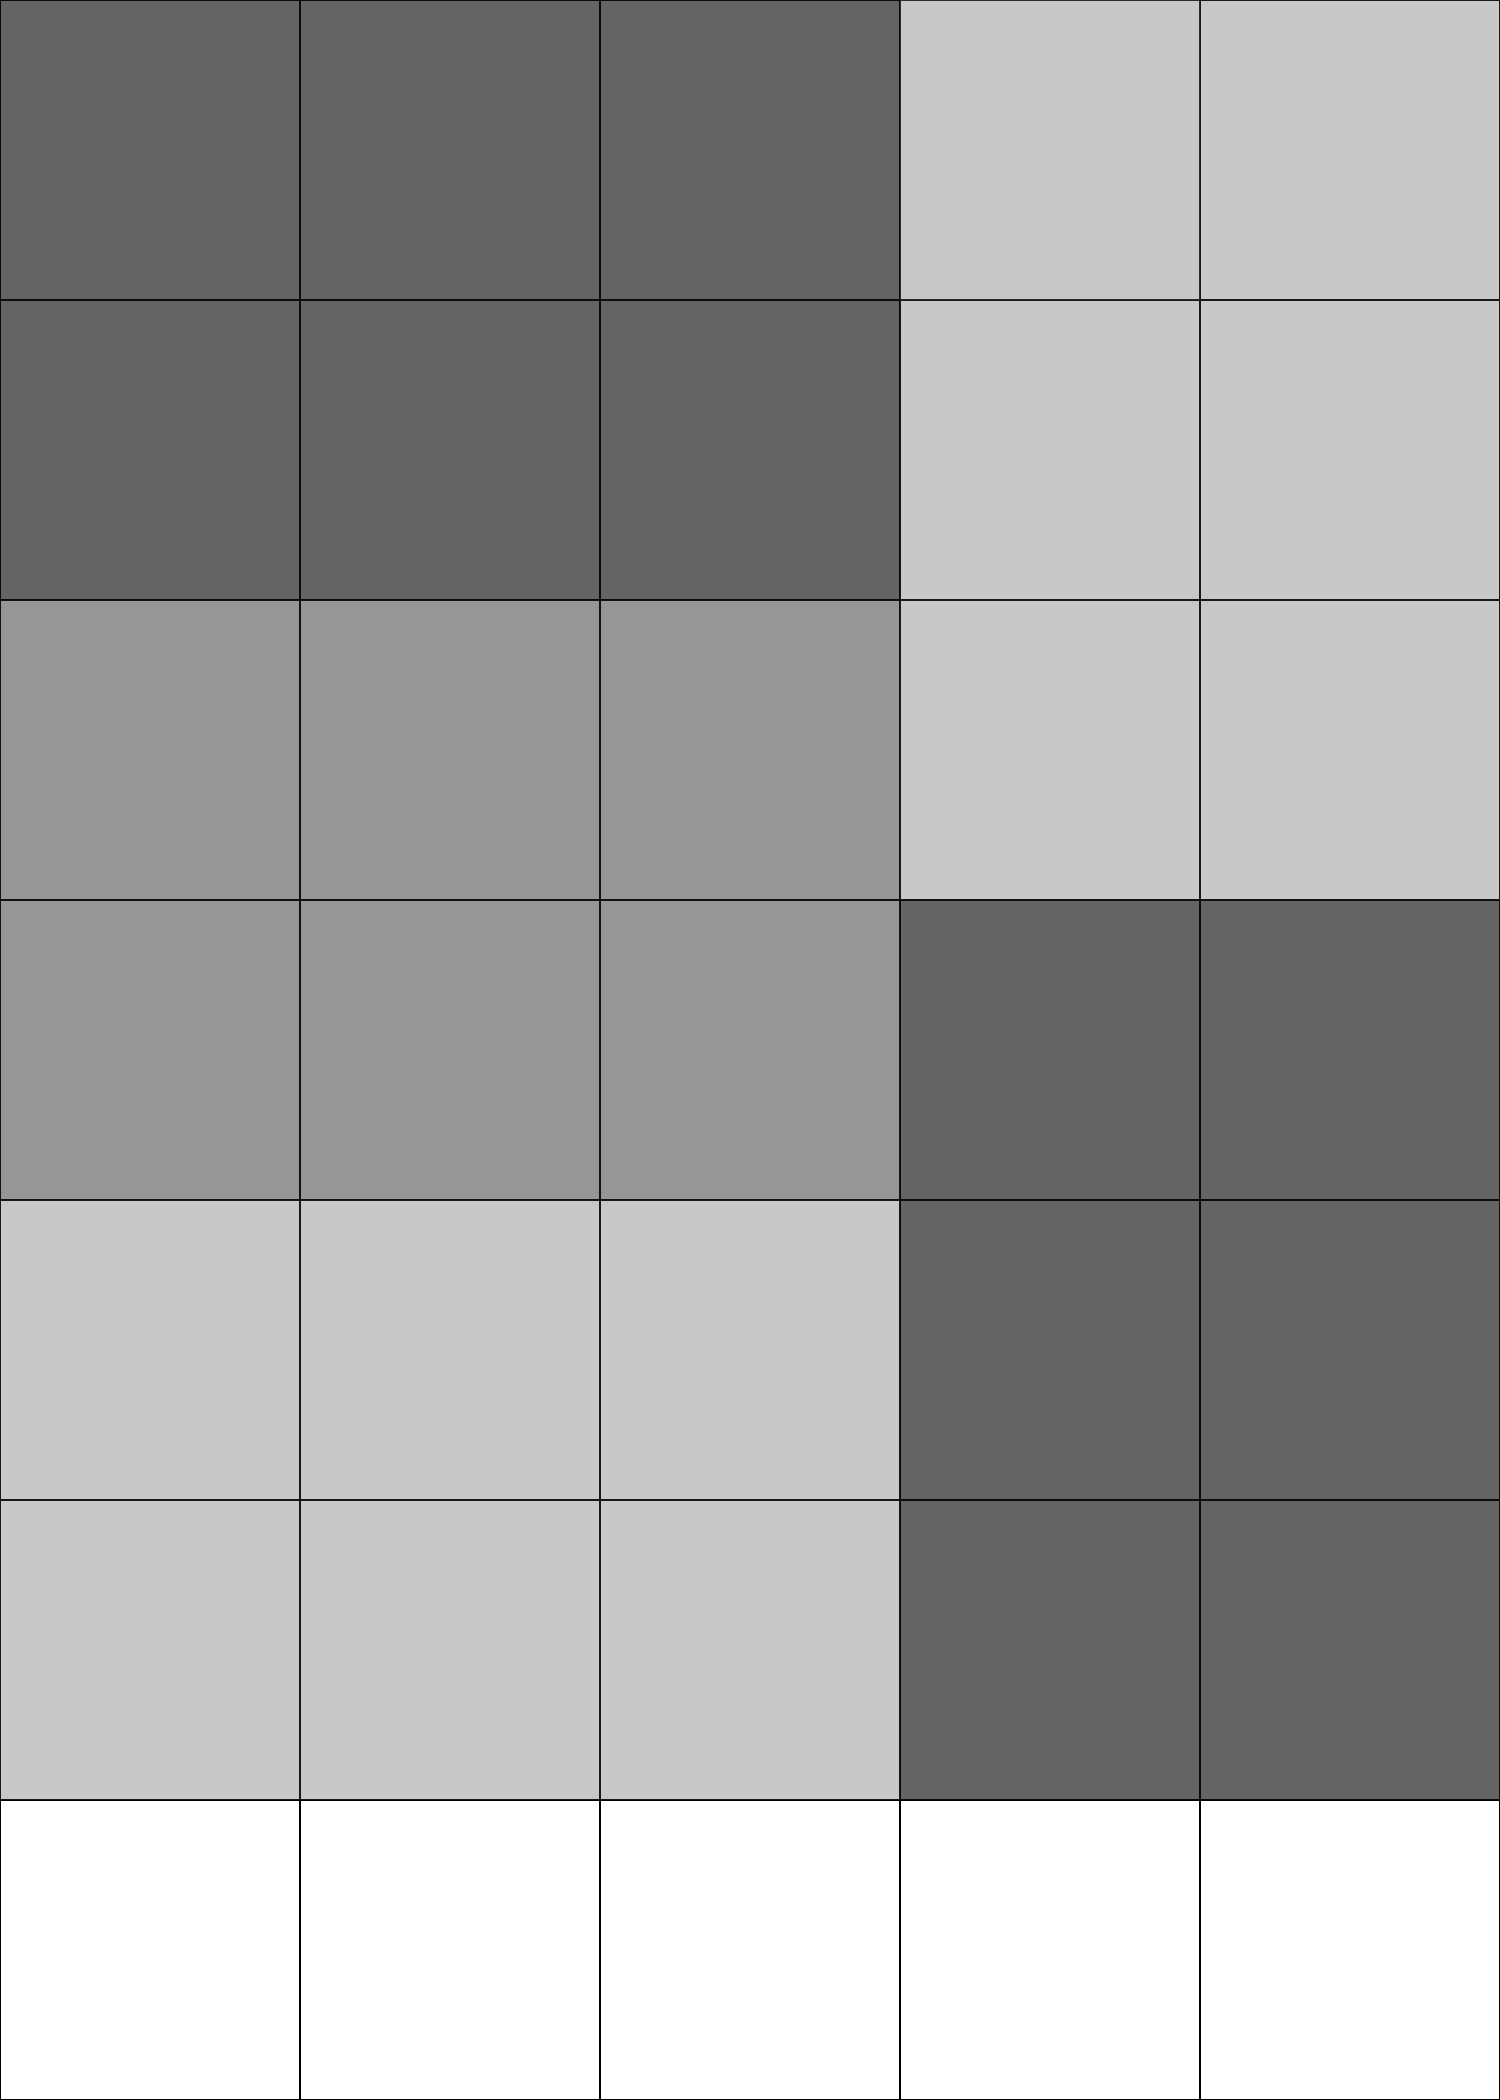
\includegraphics[height=0.68\textwidth]{pictures/5-4.png}
					\end{minipage}
					\begin{minipage}[t]{0.48\textwidth}
						\centering
						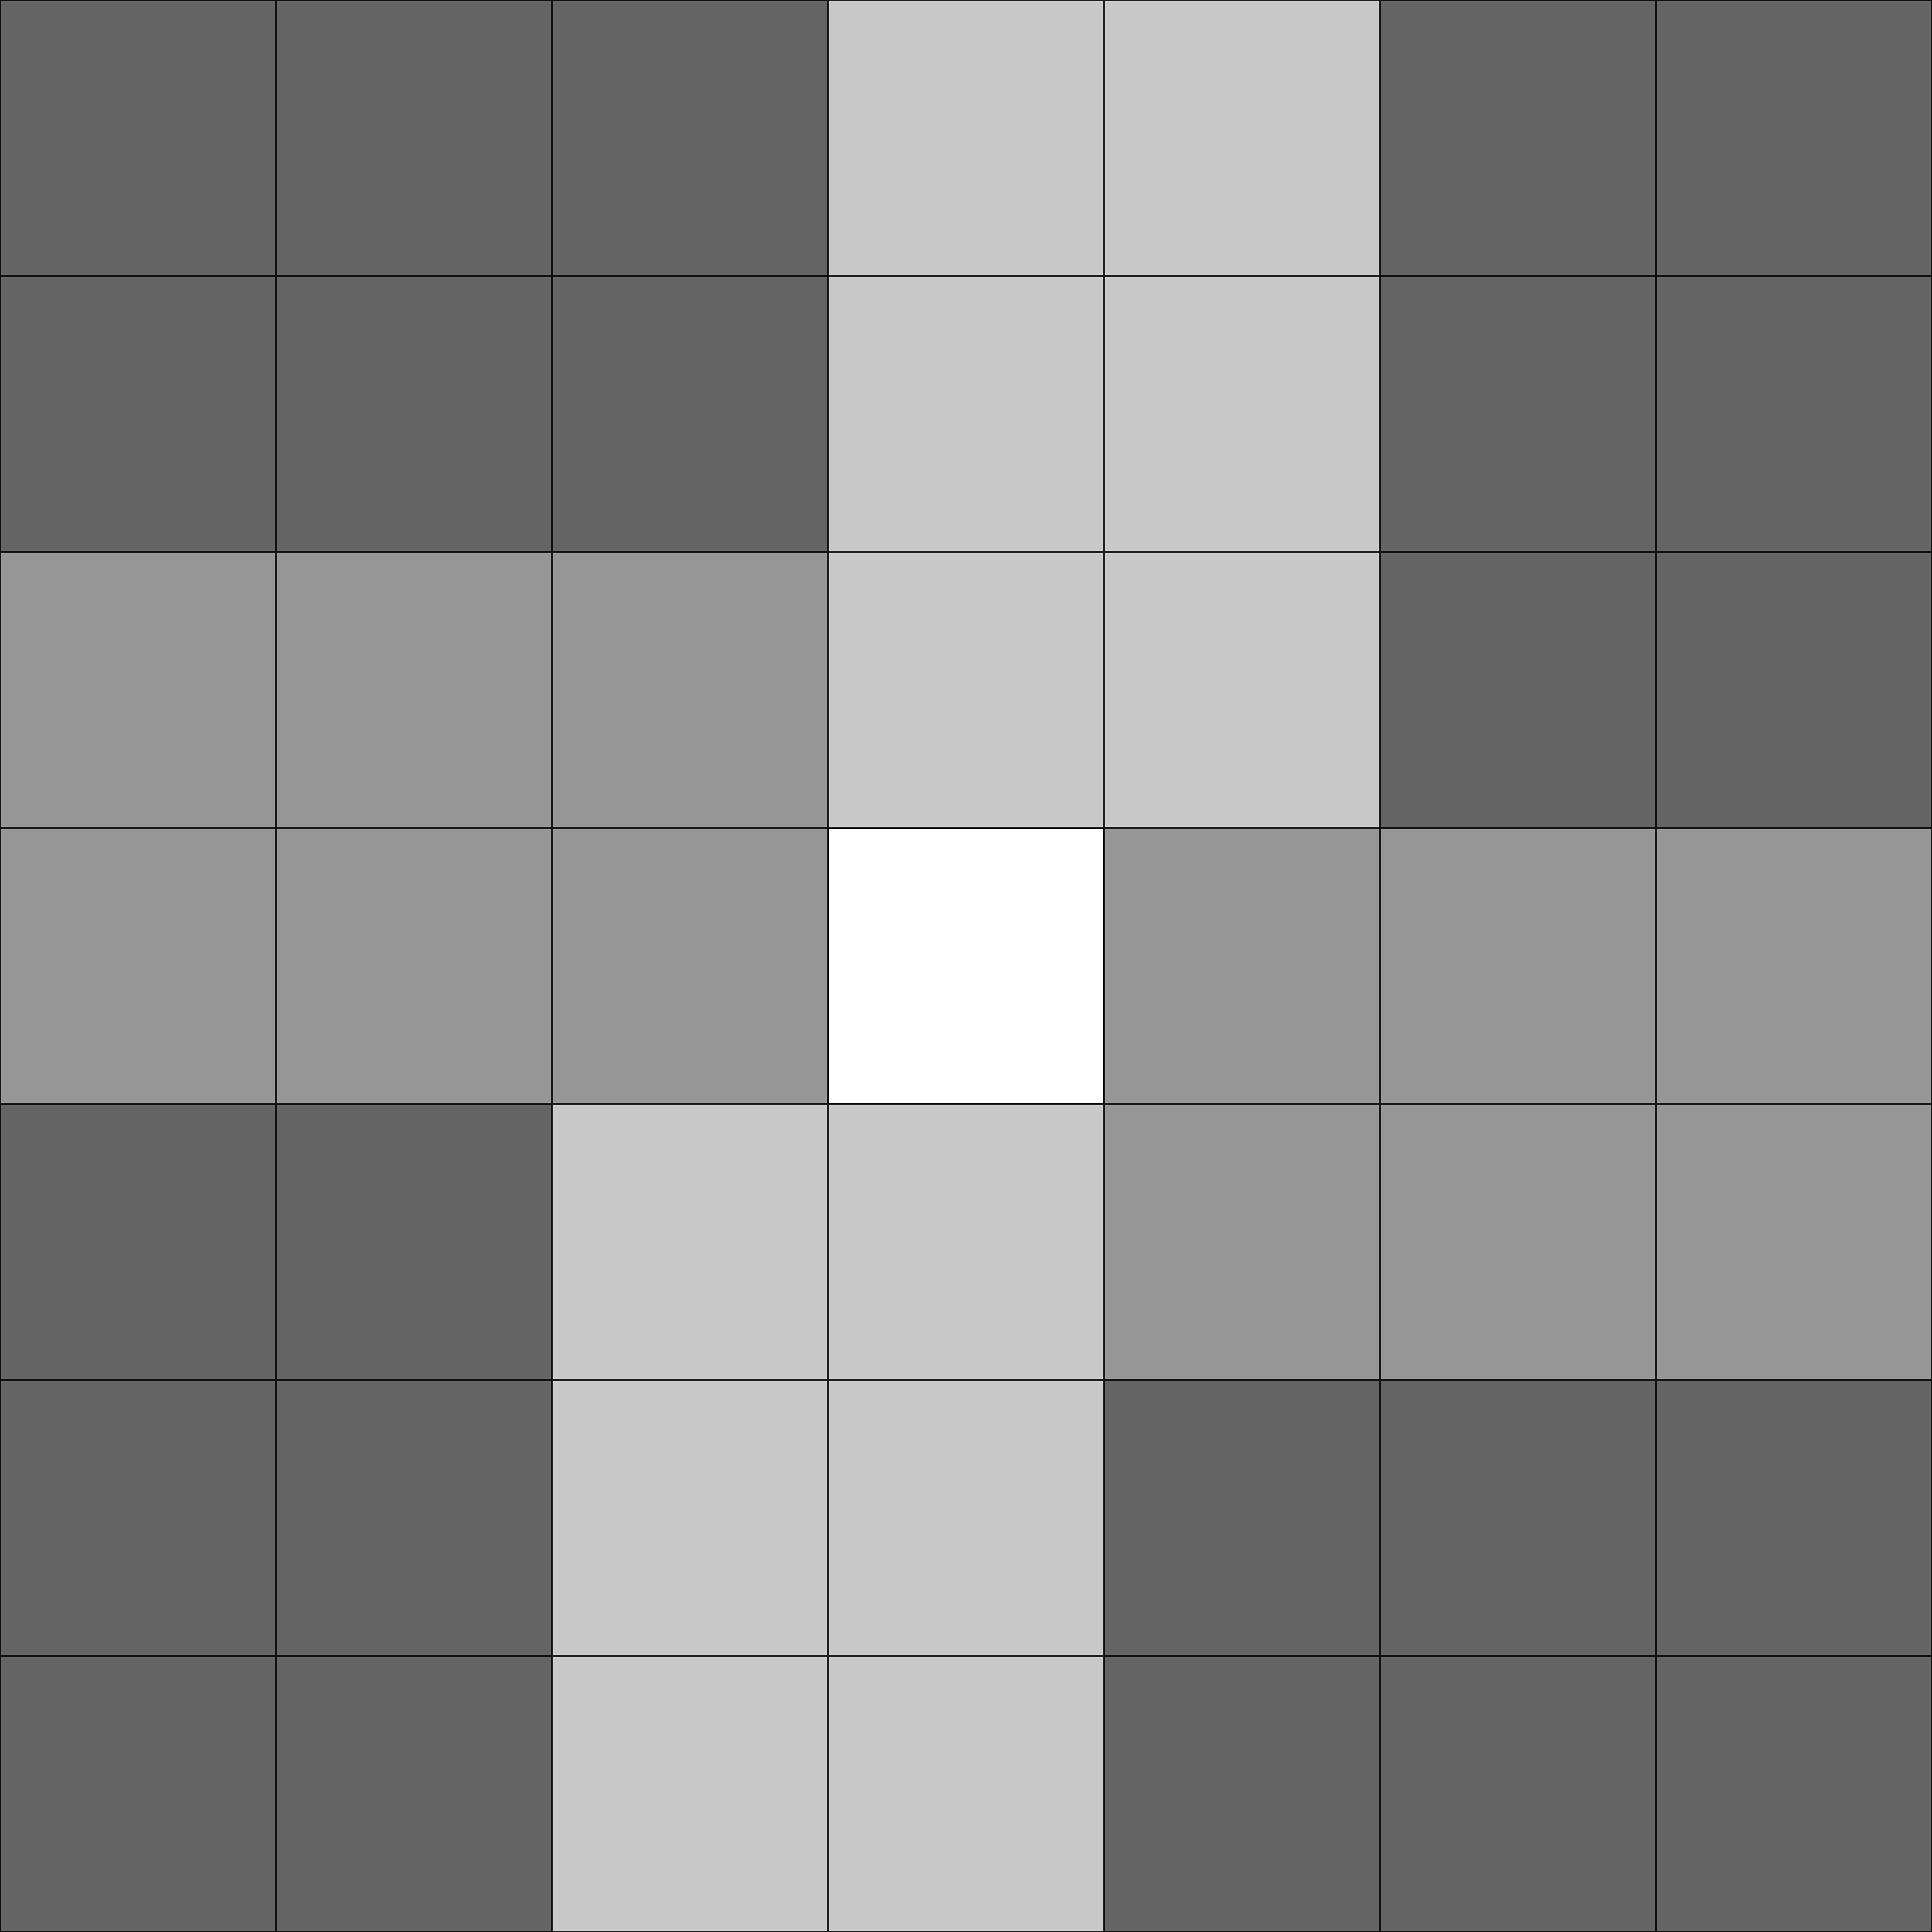
\includegraphics[height=0.68\textwidth]{pictures/5-5.png}
					\end{minipage}
				\end{figure}

				\centering{后五种情况对应的方案}
			\end{frame}
			\begin{frame}\frametitle{$r>7$时}
				由于r=6时一定可以填满,我们可以先从棋盘中划去若干列,使$2\le c\le7$,再套用上面的证明,于是这样留的空的数目一定$<6$\\
				综上所述,我们证明了对于所有的情况,都有$ans=\lfloor\frac{rc}{6}\rfloor$,即$ans=\lfloor\frac{(n+1)(m+1)}6\rfloor$
			\end{frame}
		\subsection{后记}
			\begin{frame}\frametitle{后记}
				第一题就讲完惹..\\
				HJQwQ提醒自己休息一下qwq\\
				这题本来是去年NOI之前某场CF div2的A题..当时是罕见的下午比赛,我就和机房小伙伴开黑..结果遇到了这个题\\
				我很快就证明了答案就是$\lfloor\frac{(n+1)(m+1)}{6}\rfloor$..然后一直过不了pretest..自闭了..div2A都做不出来\\
				然后比赛就被爆破(unrated)了..出题人和验题人写的是同一种乱搞做法..$n=6,m=6$时输出7..导致正解过不了pretest..\\
				然后这题就作为错题从CF题库中被删掉了..我在NOI之前错过了最后一次橙名的机会..导致橙名迟到了1年qwq
			\end{frame}
	\section{抽卡}
		\subsection{各种部分分}
			\begin{frame}\frametitle{测试点1,2}
				直接暴力dfs枚举抽的卡..然后统计答案\\
				时间复杂度大概是$O(n!)$
			\end{frame}
			\begin{frame}\frametitle{测试点3,4,5}
				动态规划..令$f_{i,j,0/1}$表示到达前$i$个位置中选了$j$个,且第$i$个选/未选的最大价值和\\
				转移方程为:\\
				$$\begin{cases}f_{i,j,0}=max(f_{i-1,j,0},f_{i-1,j,1})\\
				f_{i,j,1}=f_{i-1,j-1,0}+v_i\end{cases}$$\\
				时间复杂度$O(n^2)$
			\end{frame}
			\begin{frame}\frametitle{测试点6,7}
				$v_i$不是1就是2..大概可以乱搞?我没仔细想...
			\end{frame}
		\subsection{正解}
			\begin{frame}\frametitle{一个假贪心}
				每次抽序列中最大的..然后把它以及两侧的牌从序列中删去\\
				这样做满足了不能相邻的要求,但得到的并不是最优解..甚至抽不满$\lfloor\frac{n+1}{2}\rfloor$张卡
			\end{frame}
			\begin{frame}\frametitle{改进贪心}
				我们发现,如果$k=1$时最优解为抽$v_i$,那么$k=2$时要么抽$v_i$和另一张卡,要么抽$v_{i-1}+v_{i+1}$\\
				因为如果k=2时最优解是抽$v_{i-1}+v_j$,其中$j\neq i+1$那么说明$v_j>v_{i+1}$,且$j$与$i$不相邻,又因为$v_i$是原序列的最大值,故抽$v_i+v_j$一定优于$v_{i-1}+v_j$,矛盾\\
				抽$v_{i+1}+v_j$时同理\\
				于是由$k=1$到$k=2$的过程中,我们要么抽一张和$v_i$不相邻的卡,要么放回$v_i$,抽出$v_{i-1}$和$v{i+1}$\\
				同理,如果在$k=2$时选了$v_{i-1}+v_{i+1}$,那么$k=3$时一定再抽一张不相邻的卡,或者抽$v_{i-2}+v_i+v_{i+2}$\\
				不难发现我们每次都是在将一个类似于01010的串翻转为10101,1和0表示抽或未抽\\
			\end{frame}
			\begin{frame}\frametitle{改进贪心}
				于是我们就用堆来维护所有翻转可以获得的最大价值(可能为负),并用双向链表来维护序列\\
				每次从堆中取出一个点$v_i$,就将其加入答案,将$v_{i-1},v_i,v_{i+1}$从序列中删除,合并为一个新的点,权值为$v_{i-1}+v_{i+1}-v_i$,再插入到序列和双向链表中\\
				一共要进行$\lfloor\frac{n+1}{2}\rfloor$轮这样的操作\\
				总时间复杂度$O(n\log n)$\\
				注意特判取出的点$v_i$位于链表两端的情况,以及已经从序列中被删除的情况
			\end{frame}
		\subsection{证明}
			\begin{frame}\frametitle{证明显然(x)}
				emmm其实挺复杂的..直接感性理解就是对贪心进行了改进,可以对贪心进行反悔操作,防止陷入局部最优解..\\
				(因为证明太麻烦了所以我本来没打算出这个题..但在GGN的强烈要求下还是出了..他还立了个flag说这题没人AC他吃点啥(滑稽))\\
				\textbf{GGN巨神}给出了一个证明,课后会发给大家\\
				HJQwQ表示这题本质上是一个\textbf{模拟费用流问题},也给出了一个证明..
			\end{frame}
			\begin{frame}\frametitle{与费用流的联系}
				前置知识:网络流,费用流,MCMF算法\\
				这道题可以抽象成一个费用流问题\\
				建图方法如下..\\
				(此处有一张图片)\\
				中间的每一条边流量上限为1,费用为$v_i$,代表原来的一张卡,有流量就代表要选它\\
				左右的边流量上限为1,费用为0,保证了相邻两张卡只会选一张\\
				那么这显然就是一个最大费用流问题\\
			\end{frame}
			\begin{frame}\frametitle{与费用流的联系}
				每次$k++$的过程就是费用流的增广过程:在残量网络中找一条总费用最大的从$s$到$t$的路径,然后将这条路径的流量增加1\\
				由于总费用最大的增广路一定是从$s$到第1层节点,然后经过了若干条中间的边,最后进入$t$,这就等价于找一条翻转价值最大的01串\\
				然后将这条路径上每条边的流量+1,由于流量上限也是1,故这样会将残量网络中路径上的边反向,等价于将这个01串翻转\\
				这样就证明了题解的做法等价于费用流MCMF算法的增广过程,由于贪心沿着最长费用路增广是正确的,故题解中的也是正确的\\
				我们称这类用堆等数据结构来模拟费用流的增广/退流等操作的问题为\textbf{模拟费用流问题}\\
			\end{frame}
			\begin{frame}\frametitle{拓展}
				什么?为什么MCMF算法每次沿着最大费用路增广是正确的?\\
				时间原因这里就不再赘述..课后会发证明..有兴趣的同学可以看..
			\end{frame}
		\subsection{后记}
			\begin{frame}\frametitle{后记}
				第二题也讲完惹..\\
				HJQwQ提醒自己休息一下qwq\\
				这道题原题是\underline{\href{https://www.luogu.com.cn/problem/P1484}{洛谷P1484}}\\
				这题是我在广州集训的时候遇到的..当时还不会做..然后讲完之后觉得自己就是个锑..\\
				并且这题在很多OJ上都出现过很多次..BZOJ和洛谷至少各有3道一样的题..\\
				我能找到的最早出处大概是\underline{\href{https://www.luogu.com.cn/problem/P3620}{APIO2007数据备份}}\\
				后来就被无数集训/模拟赛/OJ抄了无数次..但极难找到这道题的正确性证明..我和\textbf{GGN巨神}证了好久才证出来\\
				总而言之是一个很经典也很有意思的题qwq\\
				STL的优先队列不开O2慢的要死..$n$只能出到$2\times10^5$..不然本来还想出到$10^6$..
			\end{frame}
	\section{归程}
		\subsection{各种部分分}
			\begin{frame}\frametitle{测试点1,2}
				可以枚举删边,然后$O(n!)$枚举所有可能的路径,再计算经过这条路径的概率和总长度,最后算出期望值\\
			\end{frame}
			\begin{frame}\frametitle{测试点3,4,5}
				令$g_i$表示从$i$号点开始走经过的路径长度期望值,则有\\
				$$g_i=\begin{cases}
					0,&\mbox{i无出边}\\
					\sum\limits_{(i,v)\in E}\frac{w_{(i,v)}}{\sum\limits_{(i,u)\in E}w_{(i,u)}}(g_v+l_{(u,v)}),&\mbox{i有出边}
				\end{cases}$$\\
				这样就可以枚举删边,然后每次用拓扑排序暴力DP,时间复杂度$O(m^2)$
			\end{frame}
			\begin{frame}\frametitle{测试点6,7}
				不太清楚有什么乱搞做法qwq..
			\end{frame}
		\subsection{正解}
			\begin{frame}\frametitle{正解}
				首先通过一次拓扑排序计算出$g_i$\\
				然后考虑删边对答案的影响:删去边$(u,v)$只会对经过$u$点的路径造成影响,并且只会对$u$点的$g$值造成影响,故要重新计算$g_u$,并求出$g_u$的变化对总答案的
				响,故我们要求出经过$u$点的概率$f_u$
				令$f_i$表示从1号点出发,前进路径经过$i$号点的概率,则有\\
				$$f_i=\begin{cases}
					1,&i=1\\
					\sum\limits_{(u,i)\in E}\frac{w_{(u,i)}}{\sum\limits_{(u,v)\in E}w_{(u,v)}}f_u,&i\neq1
				\end{cases}$$
			\end{frame}
			\begin{frame}\frametitle{正解}
				于是我们再用一次拓扑排序算出$f_i$,对一条边$(u,v)$,计算删去它后,$g_u$的变化量$\Delta g_u$,总答案$ans$的变化量$\Delta ans=\Delta g_u\times f_u$,这样算一次是$O(1)$的\\
				然后我们枚举每一条边进行计算,总答案$ans$取最小值即可,总时间复杂度$O(m)$
			\end{frame}
		\subsection{后记}
			\begin{frame}\frametitle{后记}
				终于讲完了qwq\\
				这道题原题是\underline{\href{https://darkbzoj.tk/problem/3470}{BZOJ3470}}\\
				原题要保留6位小数...我当时好像卡了好长时间的精度才过\\
				这个题也是综合了概率和期望的很妙的题..\\
				本来想出另外一道题的..但因为太容易搜到题解所以被我毙掉了\\
				然后正好想到这几天的模拟赛还没出概率期望..就想出一道概率期望\\
				本来打算出一个无向图随机游走的题..但\textbf{GGN巨神}说那种题太水了..HJQwQ就只好另外找了这道题..结果还是被\textbf{GGN巨神}秒了qwq\\
				emmm还有就是double运算不开O2好慢...本来打算出到$m\le2\times10^6$的..但试了一下直接就TLE了qwq
			\end{frame}
			\begin{frame}\frametitle{完结}
				祝大家身体健康,再见!
			\end{frame}
\end{document}